\documentclass[11pt]{article}

\usepackage[a4paper,margin=2.5cm]{geometry}
\usepackage{graphicx}
\usepackage{amsmath,amssymb,amsfonts}
\usepackage{bm}
\usepackage{textcomp}
\usepackage{booktabs}
\usepackage{array}
\usepackage{tabularx}
\usepackage{longtable}
\usepackage{multirow}
\usepackage{makecell}
\usepackage{float}
\usepackage{tikz}
\usetikzlibrary{positioning,shapes.geometric,arrows.meta,calc,fit,backgrounds,decorations.pathreplacing}
\usepackage{xcolor}
\usepackage[numbers,super,sort&compress]{natbib}
\usepackage[hidelinks]{hyperref}

\renewcommand{\citenumfont}[1]{#1}
\renewcommand{\bibnumfmt}[1]{#1.}

\newcommand{\TODO}[1]{\textbf{\textcolor{red}{[TODO: #1]}}}

\setlength{\parindent}{0pt}
\setlength{\parskip}{0.6em}

\begin{document}

\begin{center}
  {\bfseries\Large Bedside multimodal sensing for early neurological risk assessment after cardiac surgery}

  \bigskip

  Robin C.~Geyer\textsuperscript{1,2,\&,*},
  Pia Lanmueller\textsuperscript{3,\&},
  Svea Wilkending\textsuperscript{1},
  Maximilian Sch\"{o}ls\textsuperscript{4},
  Tobias R\"{o}schl\textsuperscript{3},
  Julian Madrid\textsuperscript{3},
  Matthias Hommel\textsuperscript{3},
  Benjamin O'Brien\textsuperscript{5},
  Julia Vogt\textsuperscript{2},
  Volkmar Falk\textsuperscript{3},
  Joachim M.~Buhmann\textsuperscript{2},
  Alexander Meyer\textsuperscript{1,3,*}

  \bigskip

  \begin{minipage}{0.92\textwidth}\small\raggedright
    \textsuperscript{1}Institute for Artificial Intelligence in Medicine, Charit\'{e} Universit\"atsmedizin Berlin, Berlin, Germany\\
    \textsuperscript{2}Institute for Machine Learning, ETH Zurich, Zurich, Switzerland\\
    \textsuperscript{3}Department of Cardiothoracic and Vascular Surgery, Deutsches Herzzentrum der Charit\'{e}, Charit\'{e} Universit\"atsmedizin Berlin, Berlin, Germany\\
    \textsuperscript{4}Clinic for Neurology with Experimental Neurology, Charit\'{e} Universit\"atsmedizin Berlin, Berlin, Germany\\
    \textsuperscript{5}Department of Cardiac Anesthesiology and Intensive Care Medicine, Deutsches Herzzentrum der Charit\'{e}, Charit\'{e} Universit\"atsmedizin Berlin, Berlin, Germany\\[0.4em]
    \textsuperscript{\&}These authors contributed equally.\\
    \textsuperscript{*}Corresponding authors. \TODO{add corresponding-author email addresses}
  \end{minipage}
\end{center}

\begin{center}
  \begin{minipage}{0.92\textwidth}
    \textbf{Abstract.} Neurological complications pose a high risk after cardiac surgery. Early detection is crucial for intervention, but the immediate postoperative period is clinically silent: patients remain sedated, and established risk-stratification methods are lacking. Standard electronic health record data are insufficient. A candidate biomarker for early risk is vago-sympathetic imbalance with sympathetic predominance. Two modalities capture this state independently of patient wakefulness: physiological waveforms for beat-to-beat cardiovascular dynamics, and thermo-visual imaging using peripheral vasoconstriction as a proxy. Here, we report a multimodal bedside setup acquiring these signals alongside conventional clinical data. In 154 postoperative patients (12 with neurological complications), facial thermal gradients were significantly elevated in complication cases, whereas electronic health record and waveform features lacked discriminatory power. Temporal transformer models incorporating thermo-visual imaging discriminated complications within 10 minutes of admission (area under the receiver operating characteristic curve 0.73 $\pm$ 0.04), reaching 0.79 $\pm$ 0.03 at 90 minutes. Early facial peripheral cooling associates with postoperative neurological risk, highlighting the potential of non-contact multimodal monitoring during this vulnerable window.
  \end{minipage}
\end{center}

\vspace{1ex}

% High risk of neuro comp. after cardiac surgery.
% Very hard to diagnose in PACU period.
% That's bad because earlier detection super important.
% Exisitng screening and score are insufficent, they rely on mostly on markes that become accesable only after emergence from aneastesia.

Neurological complications after cardiac surgery are associated with increased mortality, morbidity and healthcare use~\citep{arrowsmith2000central}. Early detection is crucial, as treatment-sensitive time windows narrow rapidly~\citep{saver2006time, saver2016time, selim2007perioperative}. In the immediate postoperative period, however, patients in the post-anaesthesia care unit (PACU) are typically sedated and mechanically ventilated. This creates a clinically silent window that limits neurological examination~\citep{salazar2001stroke, liu2022recent}. Deficits such as hemiparesis, seizures or delirium often only become apparent after emergence from anaesthesia. Established preoperative risk scores~\citep{euroscore2,sts2018} and bedside delirium screens~\citep{ely2001camicu,nudesc} do not provide continuous, real-time risk stratification during this interval~\citep{amundson2020timing}.

% Introduce Sympathetic predominance as a marker that might me accesbale earlier (no interaction with a at least partially awake patient is needed – AND is indicative of neuro complications! So that is a great biomarker, one that might be accesbale way before emergence from anesthesia and which might correlate with neurological compolications.
A candidate marker for early perioperative risk is sympathetic predominance. Elevated sympathetic activity occurs after cardiac surgery~\citep{hogue1994alterations, bauernschmitt2004impairment} and is linked to neurological injury, reflecting catecholamine release after cerebral ischaemia~\citep{jimenez2021cardiovascular, sposato2020post, de2015autonomic}, impaired cerebral autoregulation~\citep{chen2021autonomic, mankoo2023role, aaslid1989cerebral, lee2019dysfunctional, schramm2012impaired, longhitano2021cerebral} and inflammatory activation~\citep{mattimore2023delirium, staicu2025postoperative, hansen2025prediction, pongratz2014sympathetic, poredos2025inflammation}.

% This would have to be supported by a citation:
%Crucially, autonomic dysregulation manifests independently of the patient's wakefulness, making it a viable target for continuous monitoring during the silent PACU window.

Routine electronic health record (EHR) data do not reliably capture this dysregulation~\citep{seravalle2013assess}. To address this, we evaluated two complementary sensing modalities. First, physiological waveform data (PWF), including electrocardiography, arterial blood pressure and photoplethysmography, capturing beat-to-beat cardiovascular dynamics to estimate sympathovagal balance~\citep{colombo2015pulse, valenza2018ecg}. Second, thermo-visual imaging (TVI), capturing spatial skin-temperature gradients as a non-contact proxy for peripheral vasoconstriction and altered perfusion induced by sympathetic activation~\citep{guyenet2006sympathetic, sheng2018crosstalk}. TVI has previously shown promise in assessing peripheral haemodynamics and shock~\citep{jorge_non-contact_2021, predicting_shock_from_thermal_images, podlasek2025thermography}.
Here we systematically assess the value of these modalities for early postoperative neurological risk stratification.

\section*{Results}

We established a bedside multimodal sensing pipeline that synchronises EHR, PWF and TVI during the PACU interval (Fig.~\ref{fig:overview}).
EHR data provided low-frequency clinical measurements, laboratory values and treatment variables. PWF provided high-frequency electrocardiography, invasive arterial blood pressure and photoplethysmography. TVI provided paired thermal and visual video streams of the patient's face.

\begin{figure*}[htbp!]
  \centering
  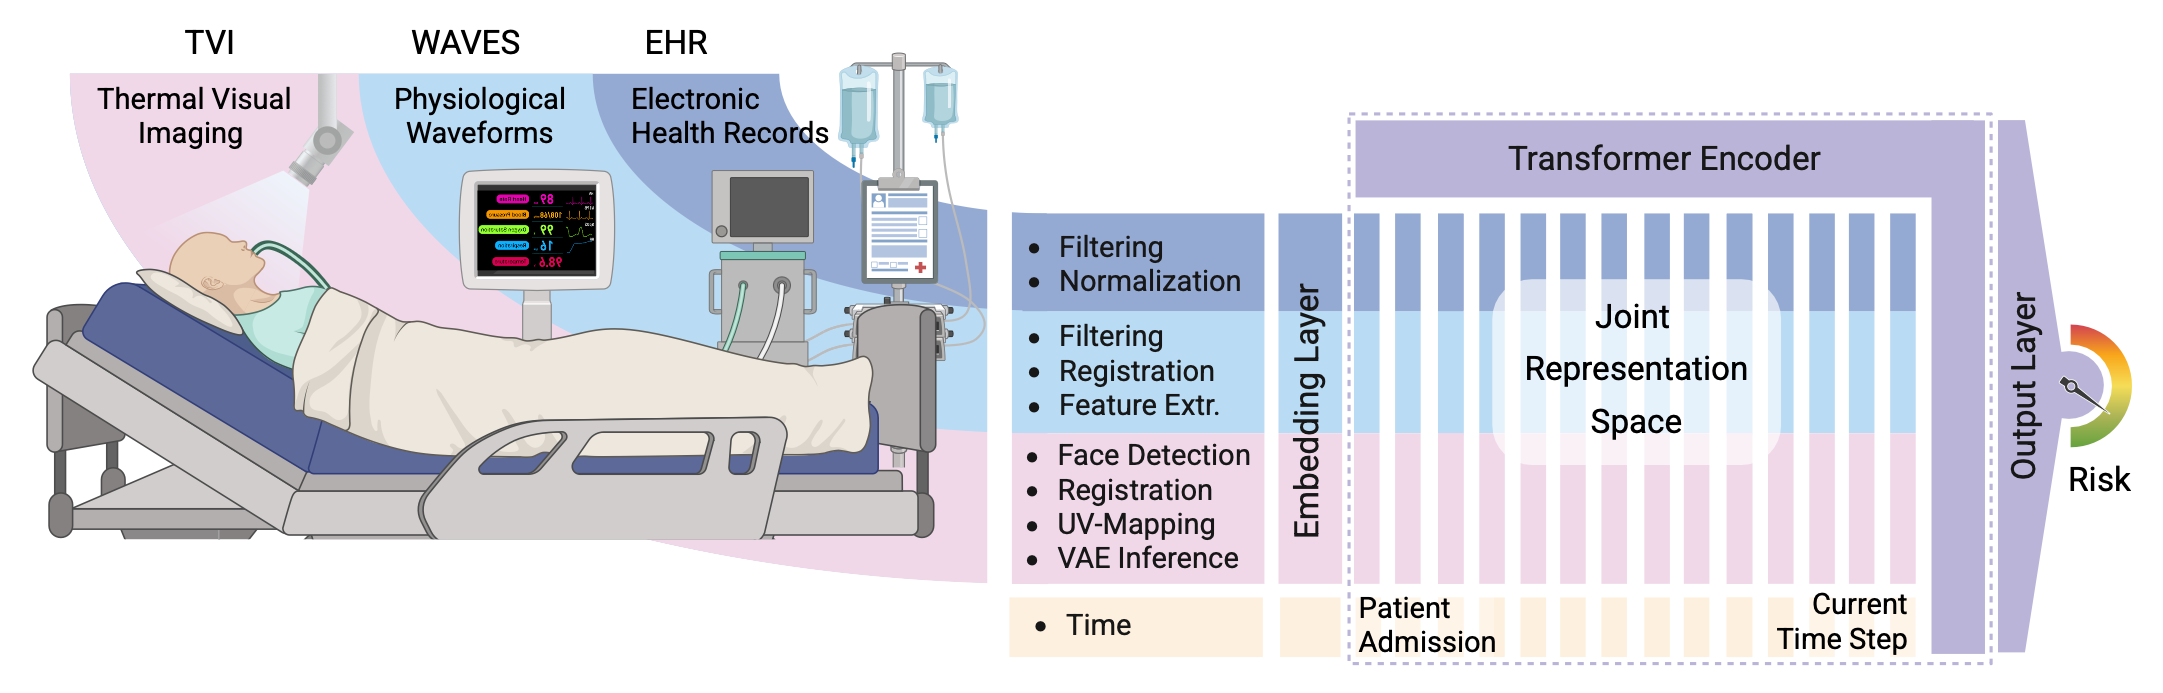
\includegraphics[width=\textwidth]{figs/Overview.png}
  \caption{Integrated bedside pipeline for early postoperative neurological risk assessment. Thermo-visual imaging (TVI), physiological waveform data (PWF) and electronic health records (EHR) are synchronised during the post-anaesthesia care unit stay. Each stream is converted into modality-specific features, embedded into a shared latent representation and processed by a temporal transformer classifier for neurological risk prediction.}
  \label{fig:overview}
\end{figure*}

Raw thermal video is high dimensional and affected by patient motion, occlusions and bedside equipment. To reduce these sources of variation, synchronised visual frames were used for three-dimensional face reconstruction, registration to the thermal frame and unwrapping into an anatomically standardised two-dimensional UV map (Fig.~\ref{fig:thermal-pipeline-vae}B). The resulting maps were encoded by a structured variational autoencoder (VAE). This isolates confounding variables such as tubes, fills in occlusions, and is trained without diagnostic labels (Fig.~\ref{fig:thermal-pipeline-vae}C,D).

\begin{figure*}[htbp!]
  \centering
  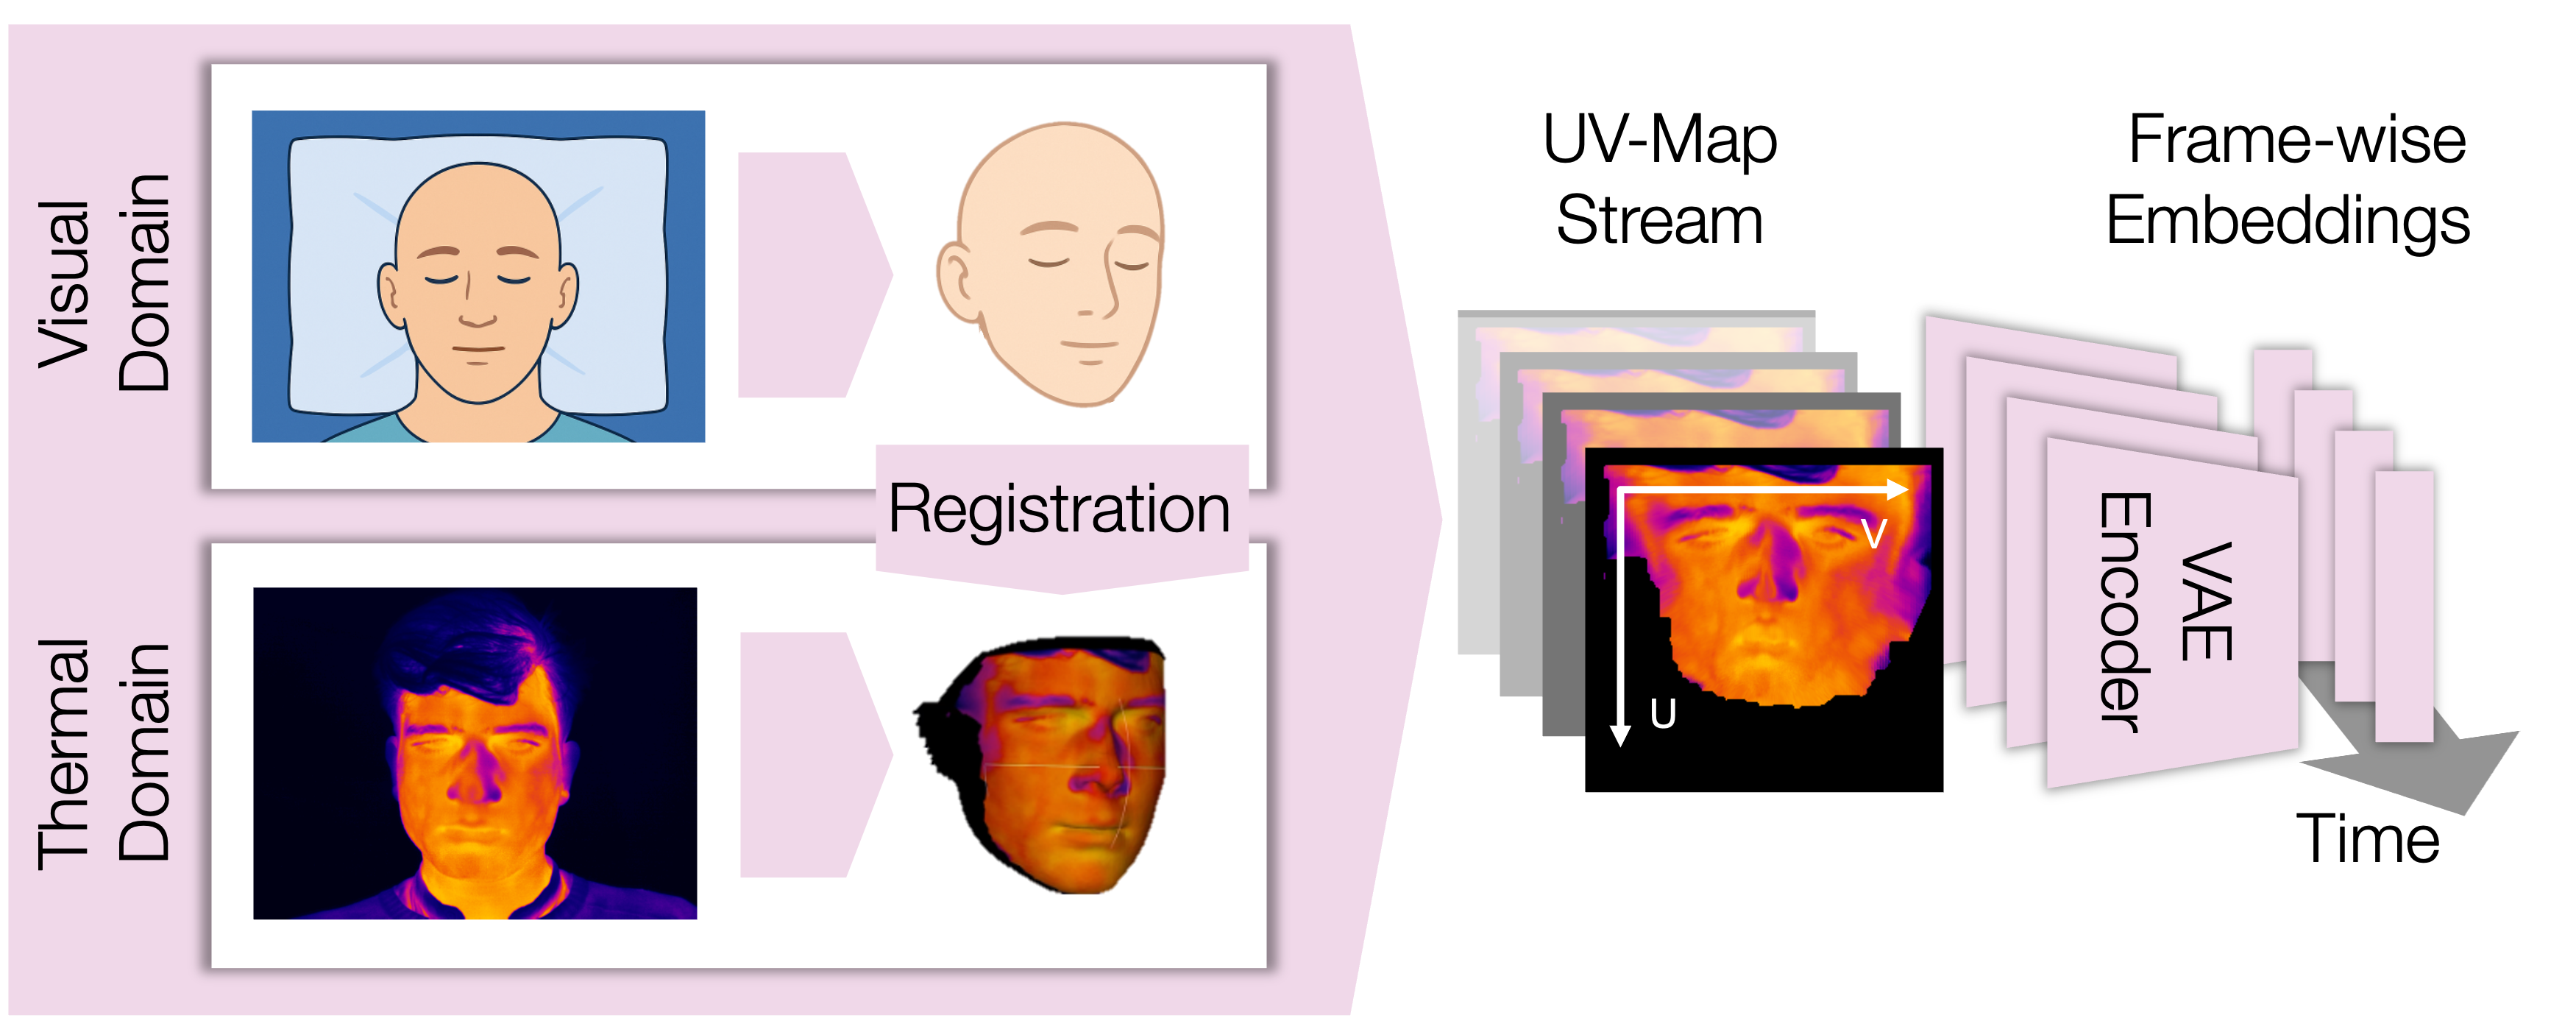
\includegraphics[width=0.5\textwidth]{figs/Thermal_pipeline.png}
  \caption{lolo}
  \label{fig:overview}
\end{figure*}


The analysis included 154 postoperative cardiac surgery patients, of whom 12 developed postoperative neurological complications. The events comprised focal neurological deficits, seizures, delirium and radiologically confirmed cerebral ischaemia or haemorrhage (case summaries are provided in the Supplementary Information). Baseline age, sex, body mass index, cardiopulmonary bypass use and surgical procedure type did not differ statistically between patients with and without neurological complications after false-discovery-rate correction (Table~\ref{tab:cohort_biomarkers}). Patients with neurological complications had longer intensive care unit and hospital stays, consistent with the clinical severity of the endpoint.

\subsection*{Thermal gradients distinguish complication cases}
EHR variables and waveform-derived haemodynamic features showed no statistically significant differences between groups after false-discovery-rate correction. Mean arterial pressure, pulse pressure and mean arterial blood pressure were similar between groups, and EHR variables including lactate, arterial blood gases, haemoglobin, creatinine, vasoactive-inotropic score, catecholamine doses and transfusion variables did not provide a corrected univariate signal (Table~\ref{tab:cohort_biomarkers}).

% I think we need to intorduce these gradients here. What is core-peripheral, and what is the other other?

In contrast, UV-standardised facial thermal gradients were statistically higher in patients with neurological complications. The core--peripheral temperature gradient was 3.39\,K [2.77, 4.31] in patients without neurological complications and 4.95\,K [4.55, 6.73] in patients with complications ($p<0.001$, $q<0.001$). The canthal--peripheral gradient was 2.77\,K [2.28, 3.25] versus 3.76\,K [3.38, 4.15] ($p=0.003$, $q=0.003$). These results indicate that facial thermal contrast, rather than routine haemodynamic or laboratory measurements, carried the strongest univariate signal in this cohort.

\begin{table*}[t]
  \caption{Selected cohort characteristics and postoperative biomarkers. Continuous variables are reported as median [interquartile range] and binary variables as $n$ (\%). P-values are from two-sided Mann--Whitney U tests for continuous variables, Fisher's exact tests for binary variables and chi-square tests for categorical variables with more than two levels. Q-values are Benjamini--Hochberg false-discovery-rate-adjusted p-values.}
  \label{tab:cohort_biomarkers}
  \centering
  \scriptsize
  \setlength{\tabcolsep}{2pt}
  \renewcommand{\arraystretch}{1.15}
  \begin{tabular}{@{}>{\raggedright\arraybackslash}p{3.0cm}>{\centering\arraybackslash}p{3.9cm}>{\centering\arraybackslash}p{3.9cm}>{\centering\arraybackslash}p{0.85cm}>{\centering\arraybackslash}p{0.85cm}@{}}
    \toprule
    \textbf{Variable} & \makecell{\textbf{No complication}\\(n=142)} & \makecell{\textbf{Neurological}\\\textbf{complication}\\(n=12)} & \textbf{p} & \textbf{q} \\
    \midrule
    \multicolumn{5}{l}{\textbf{Baseline and course}} \\
    Age, years & 64.00 [54.25, 72.00] & 72.00 [65.00, 74.75] & 0.097 & 0.243 \\
    Male sex & 101 (71.1\%) & 7 (58.3\%) & 0.344 & 0.574 \\
    ICU stay, days & 1.00 [1.00, 2.00] & 5.00 [2.75, 9.00] & <0.001 & <0.001 \\
    Hospital stay, days & 8.00 [6.00, 11.00] & 13.00 [10.00, 15.50] & 0.003 & 0.013 \\
    \midrule
    \multicolumn{5}{l}{\textbf{TVI biomarkers}} \\
    Core--peripheral gradient, K & 3.39 [2.77, 4.31] & 4.95 [4.55, 6.73] & <0.001 & <0.001 \\
    Canthal--peripheral gradient, K & 2.77 [2.28, 3.25] & 3.76 [3.38, 4.15] & 0.003 & 0.003 \\
    \midrule
    \multicolumn{5}{l}{\textbf{PWF biomarkers}} \\
    MAP variability, mmHg & 1.71 [1.23, 2.46] & 2.11 [1.62, 2.43] & 0.266 & 0.799 \\
    Pulse pressure, mmHg & 48.62 [40.17, 60.89] & 48.62 [42.83, 56.38] & 0.891 & 0.891 \\
    \midrule
    \multicolumn{5}{l}{\textbf{Selected EHR biomarkers}} \\
    Lactate, mmol/l & 7.00 [6.00, 11.00] & 7.00 [6.00, 10.25] & 0.752 & 0.799 \\
    Haemoglobin, g/dl & 11.40 [10.30, 12.40] & 10.70 [9.88, 11.30] & 0.047 & 0.664 \\
    Vasoactive-inotropic score & 6.00 [4.00, 12.00] & 8.00 [7.75, 13.25] & 0.141 & 0.664 \\
    Norepinephrine, \textmu g/kg/min & 0.06 [0.04, 0.10] & 0.08 [0.07, 0.09] & 0.188 & 0.664 \\
    \bottomrule
  \end{tabular}
\end{table*}

\clearpage

\subsection*{Thermo-visual imaging improves early risk stratification}

To evaluate the predictive value of multimodal sensing, transformer-based classifiers were trained on all seven modality combinations using 12-fold cross-validation across seven random seeds, with each fold containing one neurological complication case. Each modality was projected through learned embedding layers into a shared latent space. The transformer processed sequential samples from admission up to the prediction time to output a binary neurological risk prediction. Data splits for the thermo-visual variational autoencoder were strictly matched across all modality combinations.

Model discrimination was assessed using the area under the receiver operating characteristic curve (AUROC), a robust primary metric for strongly imbalanced cohorts~\citep{mcdermott2024closer}. Models relying solely on EHR, PWF, or their combination (EHR+PWF) yielded near-chance AUROC values across the early observation window (Table~\ref{tab:results_by_time}). Conversely, every modality combination incorporating TVI achieved higher discrimination. At 10\,min after PACU admission, the trimodal model reached an AUROC of 0.73 $\pm$ 0.04, compared with 0.55 $\pm$ 0.03 for EHR, 0.51 $\pm$ 0.03 for PWF and 0.70 $\pm$ 0.03 for TVI alone. At 90\,min, the trimodal model reached an AUROC of 0.79 $\pm$ 0.03, while TVI alone achieved 0.77 $\pm$ 0.02. Across the observation window, AUROC trajectories and ROC curves demonstrated consistent performance separation between models with and without TVI (Fig.~\ref{fig:auroc-roc}).

\begin{table*}[t]
  \caption{
    AUROC from 10 to 90 min after PACU admission for all combinations of EHR, physiological waveforms (PWF), and thermo-visual imaging (TVI). Values are mean $\pm$ s.d. across seven random seeds. The highest mean AUROC in each row is shown in bold.
  }
  \label{tab:results_by_time}
  \centering
  \footnotesize
  \setlength{\tabcolsep}{2pt}
  \renewcommand{\arraystretch}{1.08}
  \begin{tabularx}{\textwidth}{@{}l*{7}{>{\centering\arraybackslash}X}@{}}
    \toprule
    \textbf{Time} &
    \textbf{EHR} &
    \makecell{\textbf{EHR}\\\textbf{+ PWF}} &
    \textbf{PWF} &
    \textbf{TVI} &
    \makecell{\textbf{TVI}\\\textbf{+ EHR}} &
    \makecell{\textbf{TVI}\\\textbf{+ PWF}} &
    \makecell{\textbf{All}\\\textbf{modalities}} \\
    \midrule
    10m &
    0.55 $\pm$ 0.03 &
    0.57 $\pm$ 0.04 &
    0.51 $\pm$ 0.03 &
    0.70 $\pm$ 0.03 &
    0.71 $\pm$ 0.03 &
    0.70 $\pm$ 0.02 &
    \textbf{0.73 $\pm$ 0.04} \\

    20m &
    0.57 $\pm$ 0.03 &
    0.57 $\pm$ 0.04 &
    0.49 $\pm$ 0.03 &
    0.72 $\pm$ 0.03 &
    0.73 $\pm$ 0.03 &
    0.71 $\pm$ 0.02 &
    \textbf{0.74 $\pm$ 0.04} \\

    30m &
    0.59 $\pm$ 0.04 &
    0.58 $\pm$ 0.04 &
    0.49 $\pm$ 0.03 &
    0.73 $\pm$ 0.03 &
    0.74 $\pm$ 0.03 &
    0.73 $\pm$ 0.03 &
    \textbf{0.75 $\pm$ 0.04} \\

    60m &
    0.62 $\pm$ 0.03 &
    0.59 $\pm$ 0.04 &
    0.51 $\pm$ 0.04 &
    0.75 $\pm$ 0.02 &
    0.77 $\pm$ 0.03 &
    0.75 $\pm$ 0.03 &
    \textbf{0.78 $\pm$ 0.03} \\

    90m &
    0.63 $\pm$ 0.04 &
    0.60 $\pm$ 0.04 &
    0.49 $\pm$ 0.02 &
    0.77 $\pm$ 0.02 &
    0.78 $\pm$ 0.02 &
    0.77 $\pm$ 0.03 &
    \textbf{0.79 $\pm$ 0.03} \\
    \bottomrule
  \end{tabularx}
\end{table*}

\begin{figure*}[htbp]
  \centering
  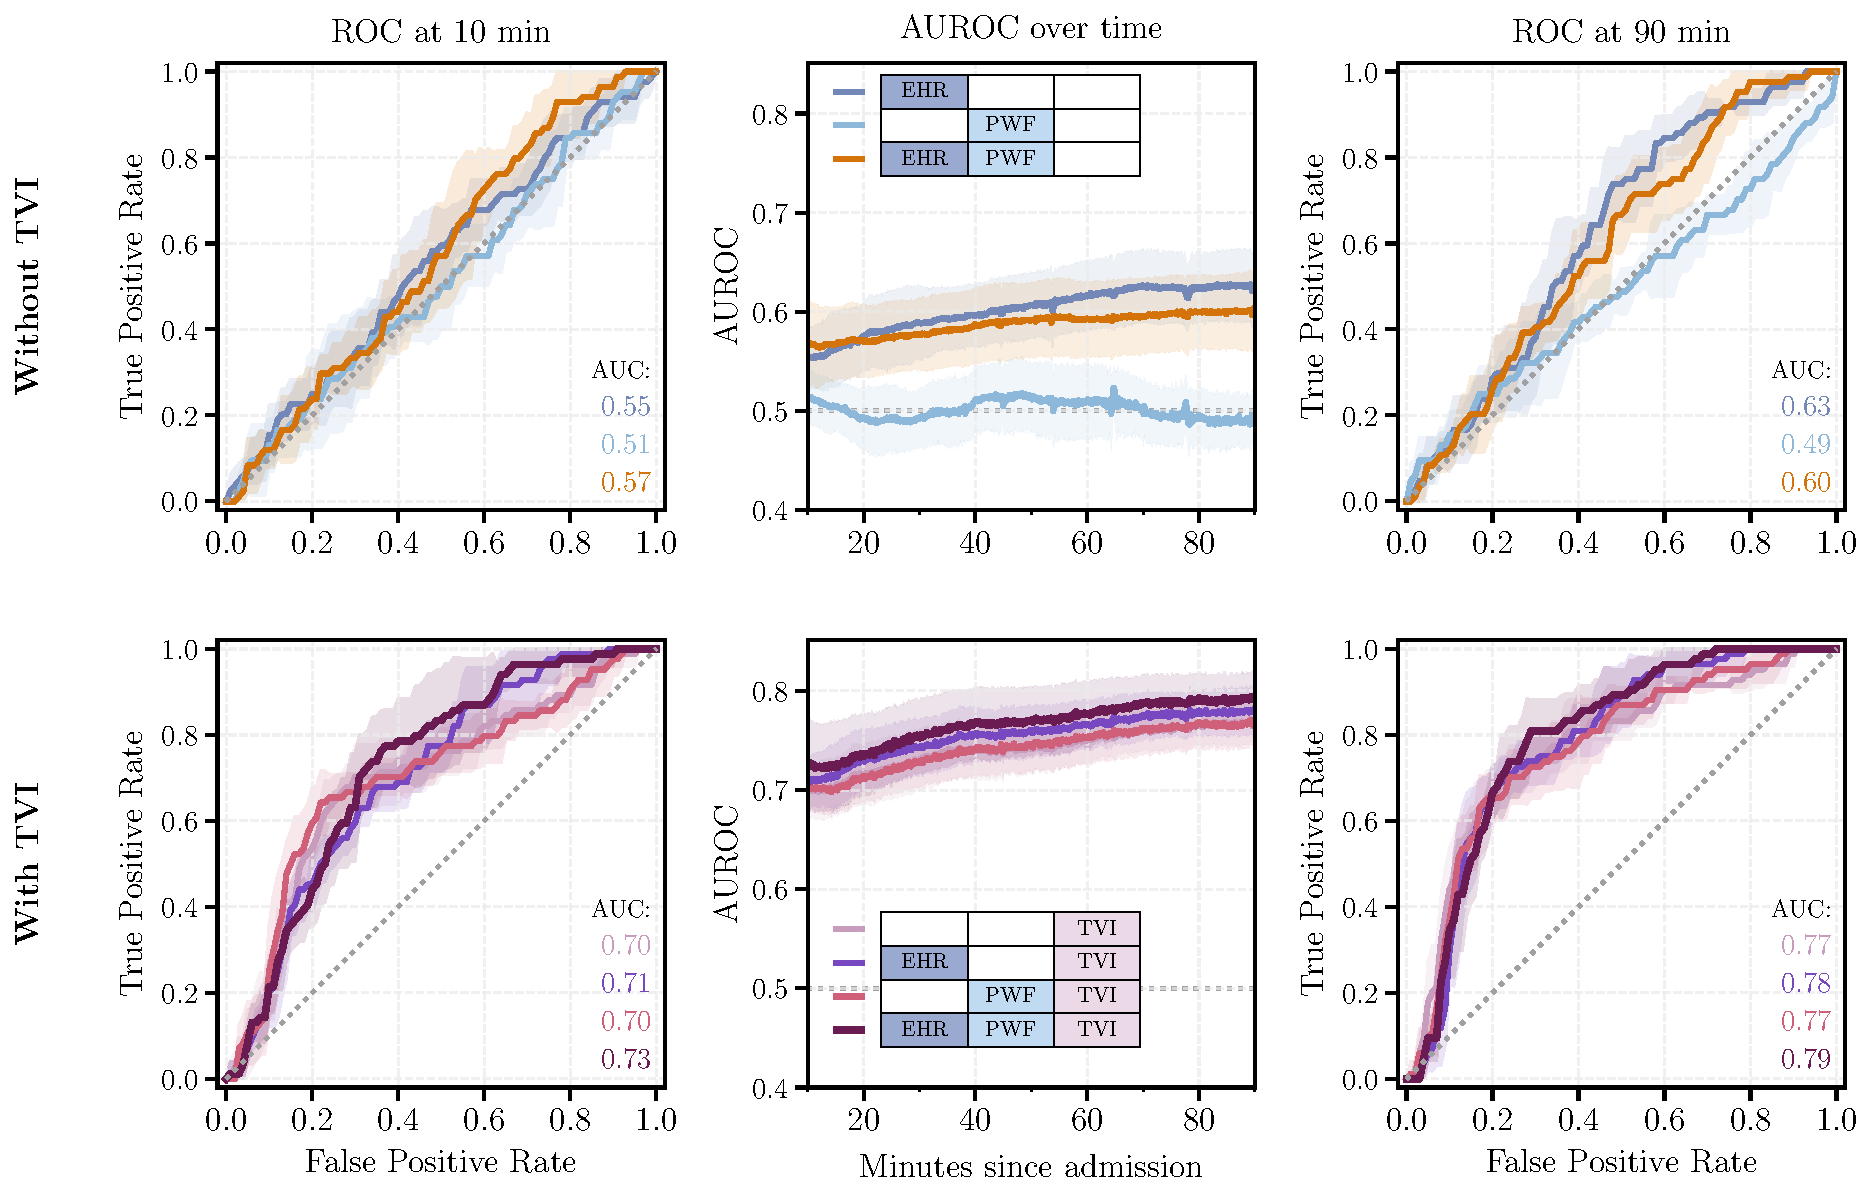
\includegraphics[width=0.95\textwidth]{figs/auroc_and_roc_combined.pdf}
  \caption{Discrimination performance across modality combinations. Models were trained with all combinations of electronic health records (EHR), physiological waveform data (PWF) and thermo-visual imaging (TVI). Receiver operating characteristic curves are shown at 10 and 90\,min after post-anaesthesia care unit admission. AUROC trajectories summarize discrimination from 10 to 90\,min. Values are based on 12 neurological complication cases and 142 controls; summary statistics across random seeds are provided in Table~\ref{tab:results_by_time}.}
  \label{fig:auroc-roc}
\end{figure*}

Risk ranks showed the same pattern. At 90\,min, the mean relative risk rank across complication cases was 0.77 $\pm$ 0.03 for the trimodal model and 0.75 $\pm$ 0.02 for the TVI-only model, compared with 0.62 $\pm$ 0.03 for EHR, 0.49 $\pm$ 0.05 for PWF and 0.59 $\pm$ 0.03 for EHR+PWF. The temporal rank trajectories showed that TVI-containing models placed many neurological complication cases among the highest-risk patients from the earliest timepoints, whereas models without TVI were less consistent (Fig.~\ref{fig:patient-ranks}). An encoder ablation, replacing the structured VAE with a vanilla VAE while keeping all three modalities active, reduced 90-min AUROC from 0.79 $\pm$ 0.03 to 0.71 $\pm$ 0.03 (Supplementary Information).

To estimate practical utility for early warning, we evaluated the models at a fixed sensitivity of 66.7\% (detecting 8 out of 12 complications). At this threshold, the TVI-only model achieved a positive predictive value (PPV) of 23.3\% at 20\,min and 26.2\% at 90\,min, corresponding to 3.4 and 2.9 false alarms per true alarm, respectively. By comparison, the EHR-only model achieved a PPV of 10.7\% at 20\,min and 11.5\% at 90\,min, producing 8.6 and 7.8 false alarms per true alarm, respectively.

\begin{figure*}[htbp]
  \centering
  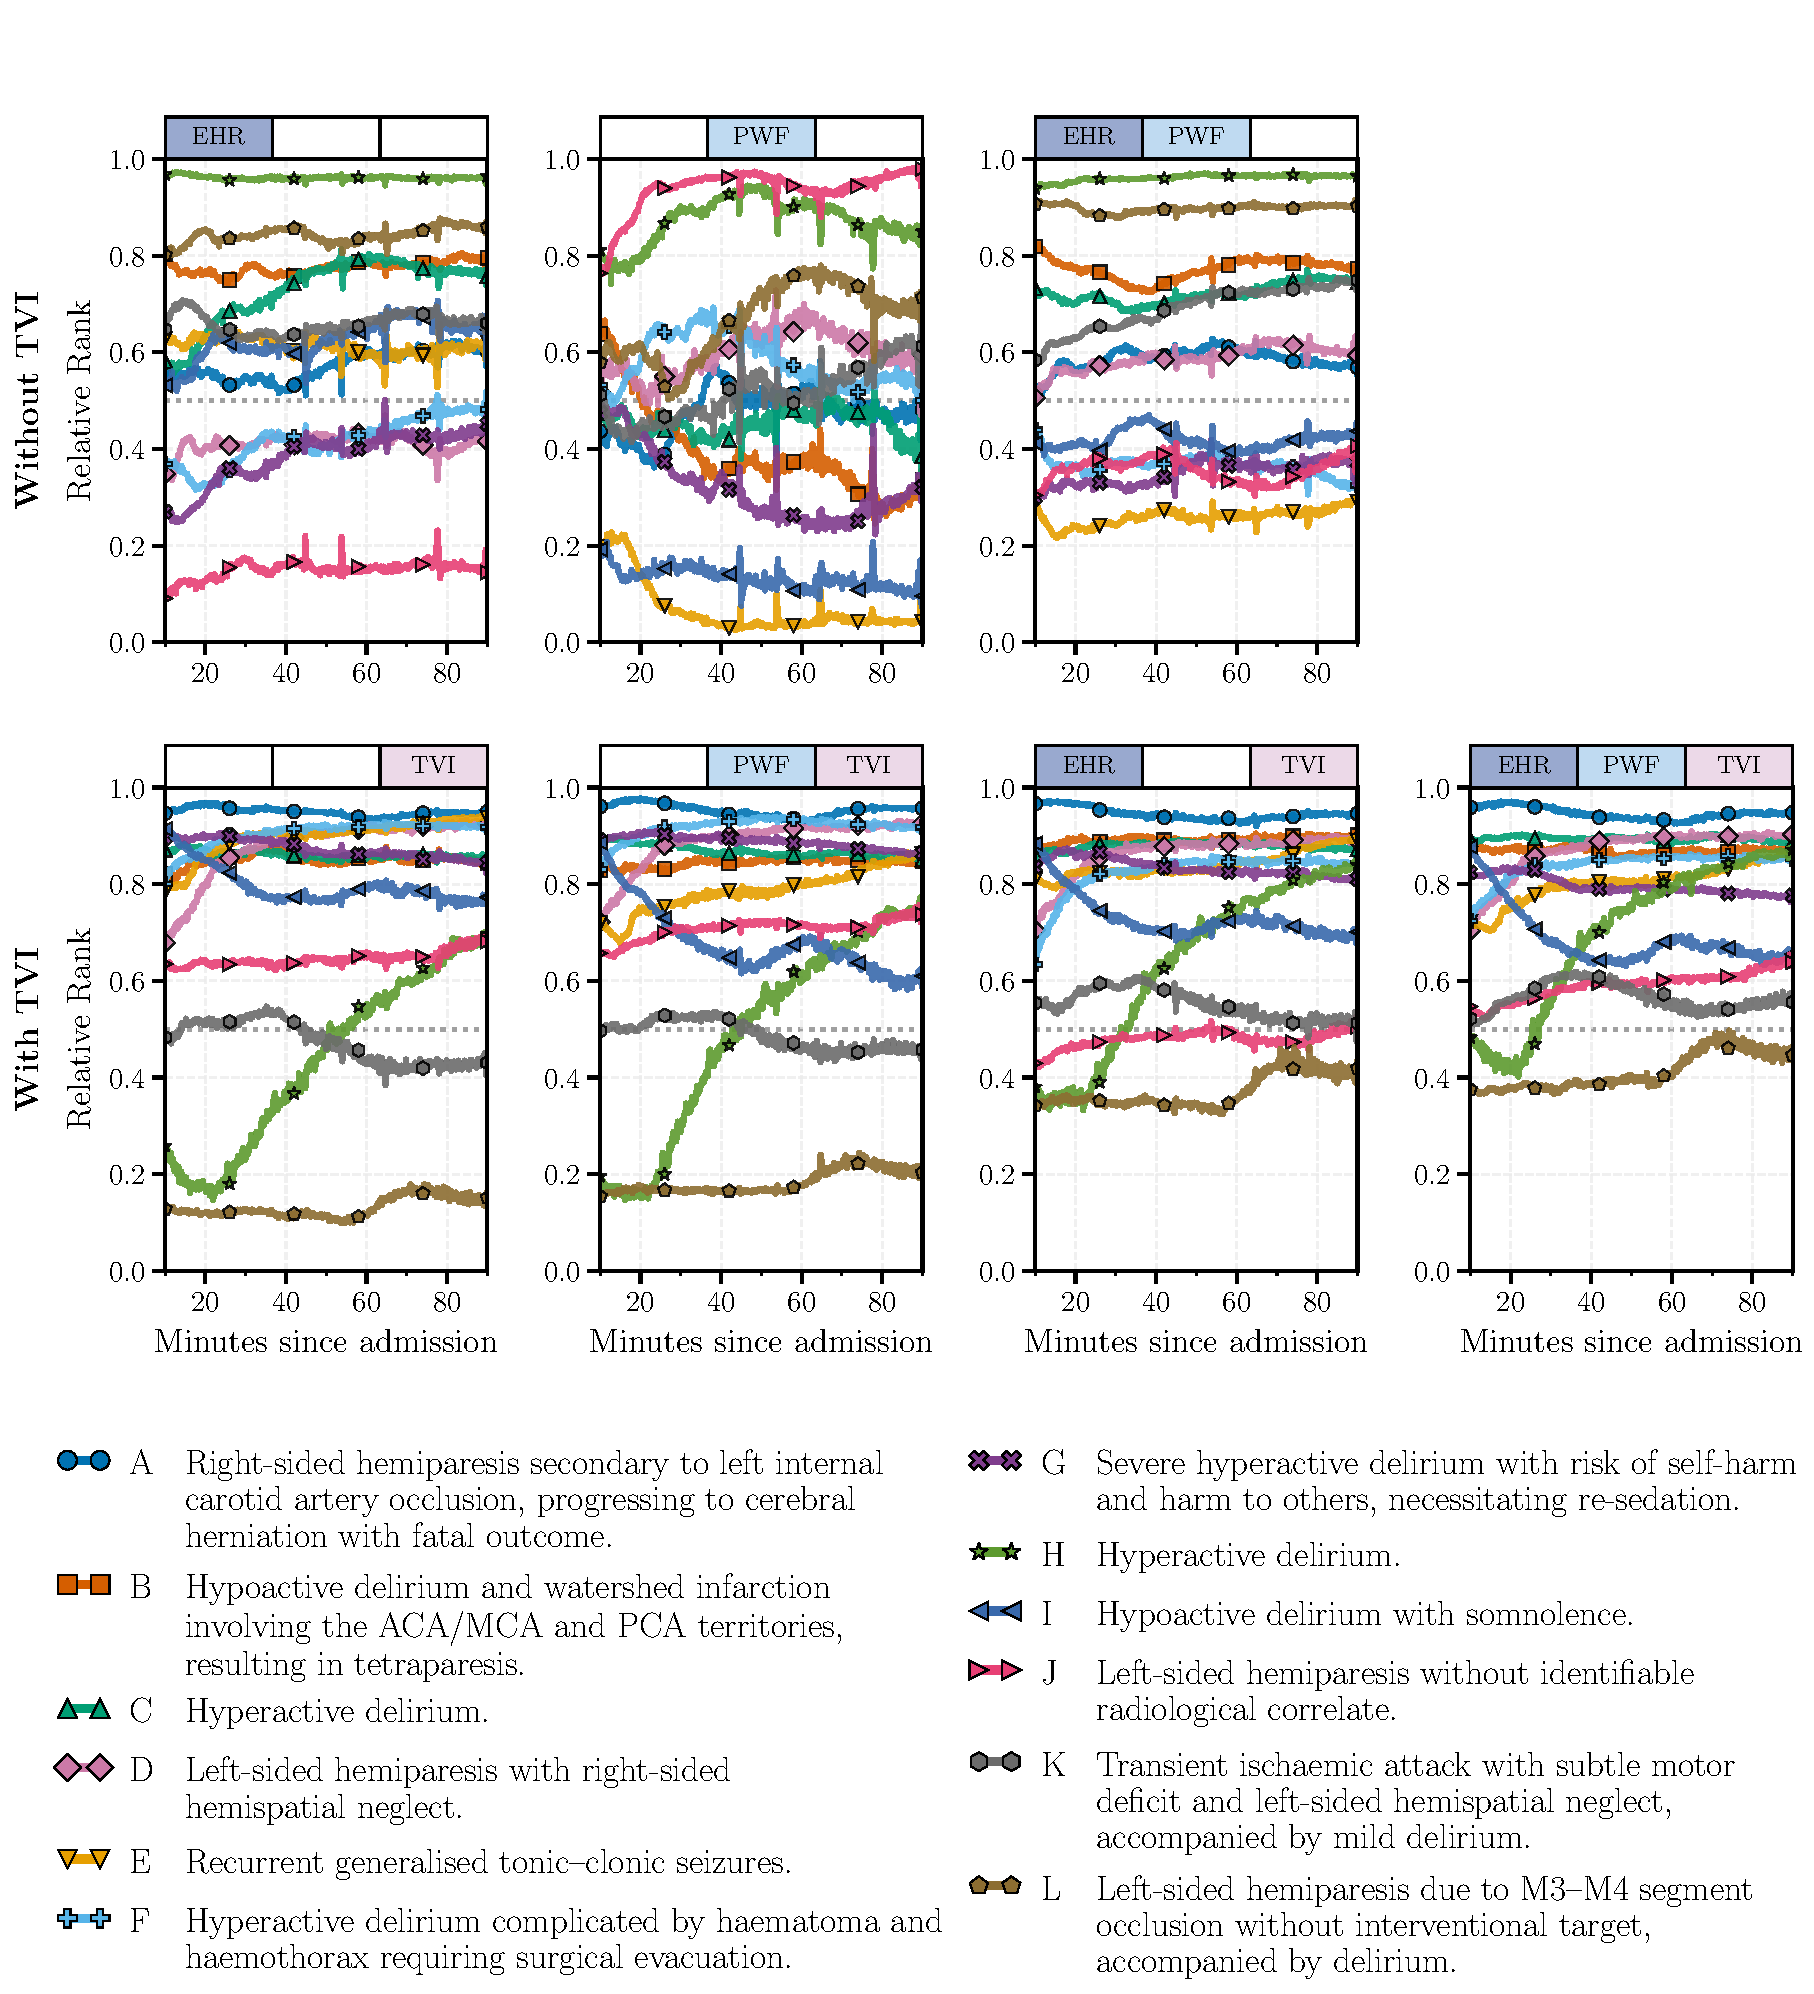
\includegraphics[width=\textwidth]{figs/patient_ranks_over_time.pdf}
  \caption{Temporal evolution of patient risk ranks during the early postoperative period. Each line traces the relative risk rank assigned to an individual patient with a neurological complication across time for a model trained on a specific modality combination. Higher values denote a higher model-assigned risk rank. Curves summarize 12 biological cases with neurological complications across cross-validation folds and random seeds.}
  \label{fig:patient-ranks}
\end{figure*}

\subsection*{Thermal maps suggest altered peripheral perfusion}

UV-standardised thermal maps showed lower peripheral facial temperatures in patients with neurological complications, particularly over the nose and cheeks, while bladder-derived core temperature followed a similar warming trajectory in both groups (Fig.~\ref{fig:neuro-temp}). The preserved core-temperature pattern argues against systemic hypothermia as the sole explanation and is compatible with altered peripheral facial perfusion.

The patients with neurological complications were not enriched for higher vasoactive-inotropic score, catecholamine dose or transfusion exposure after correction for multiple comparisons (Table~\ref{tab:cohort_biomarkers}). These descriptive analyses do not establish a causal mechanism, but they suggest that the TVI signal was not simply a surrogate for routinely documented haemodynamic support intensity.

\begin{figure*}[htbp]
  \centering
  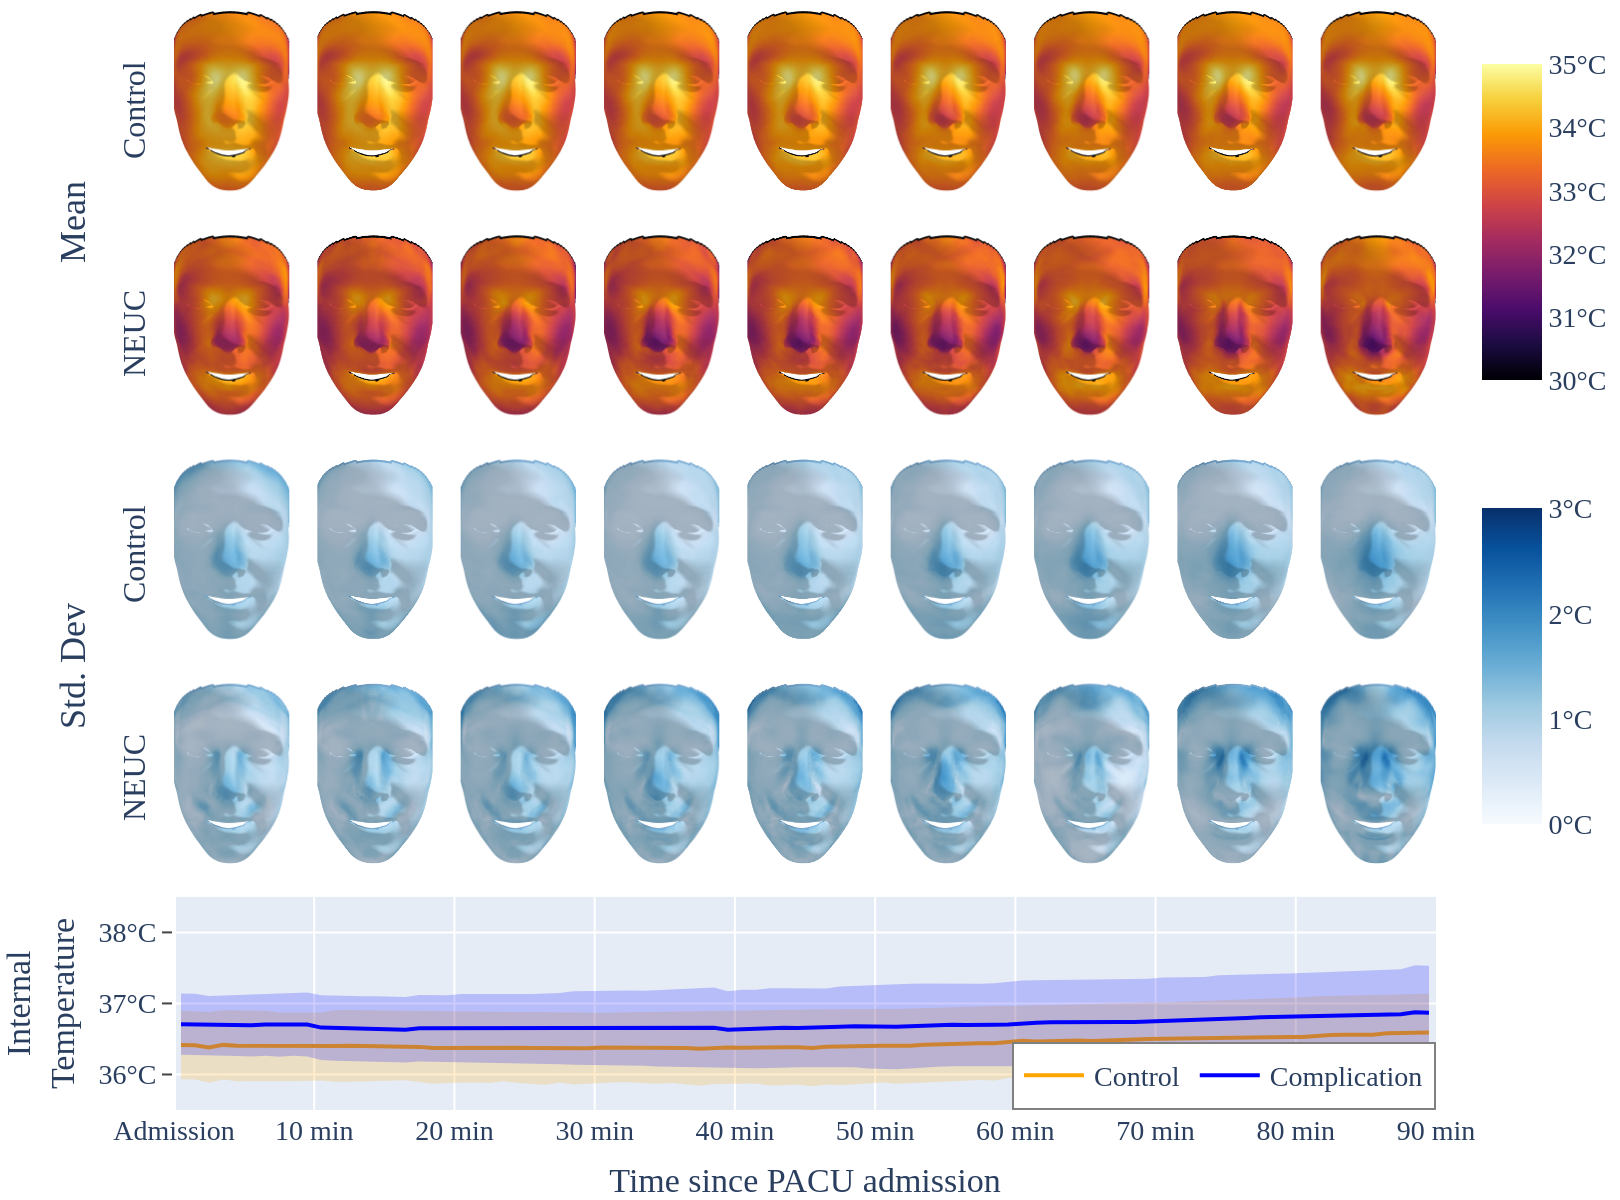
\includegraphics[width=\textwidth]{figs/thermal_evolution_neuro_means.png}
  \caption{Facial thermal maps over the first 3\,h in the post-anaesthesia care unit for patients with and without postoperative neurological complications. Rows 1 and 2 show mean facial temperature maps for controls (n=142) and complication cases (n=12) across consecutive 15-min intervals. Rows 3 and 4 show the corresponding standard deviations across patients. Row 5 shows bladder-derived core temperature, reported as the mean trajectory for each group. Temperature values are shown in kelvin where applicable.}
  \label{fig:neuro-temp}
\end{figure*}

\section*{Discussion}

This study associates early postoperative facial thermal patterns with neurological complications after cardiac surgery. In a cohort of 154 patients, TVI-derived facial temperature gradients differed between patients with and without neurological complications, whereas routine EHR variables and waveform-derived haemodynamic features did not show corrected univariate differences. In temporal prediction models, modality combinations containing TVI discriminated neurological complications from the first 10\,min after PACU admission and ranked complication cases higher than models trained only on EHR or PWF data.

The main physiological observation was a pattern of peripheral facial cooling with preserved core temperature. Because sedated and mechanically ventilated patients cannot be examined neurologically, this interval is clinically important: risk information that is available before emergence from anaesthesia could support closer monitoring and prioritization for neurological assessment. The present data do not show that thermal imaging diagnoses neurological injury, nor do they define an intervention threshold. Rather, they indicate that non-contact facial thermometry contains information associated with neurological risk that is not captured by the routine variables evaluated here.

One possible interpretation is that the thermal phenotype reflects autonomic or microvascular changes related to perioperative neurological injury. Sympathetic activation, impaired cerebral autoregulation, inflammation and catecholamine release have all been implicated in neurological complications and can influence peripheral perfusion. The observation that the strongest differences occurred in peripheral facial regions, rather than in bladder-derived core temperature, is consistent with this interpretation. However, the endpoint was clinically heterogeneous, including ischaemic events, seizures and delirium, and the shared thermal pattern should therefore be interpreted as a risk-associated phenotype rather than a single disease-specific mechanism.

The study has limitations. It was performed at a single tertiary cardiac centre, with 12 neurological complication cases, and the models were evaluated retrospectively. Although cross-validation was designed to keep one complication case per fold and was repeated across random seeds, external validation is required to quantify generalisation across institutions, surgical case mix, camera placement, ventilation practices and postoperative workflows. The neurological endpoint was based on clinically recognised complications; subclinical events may have been missed. The acquisition system required synchronised imaging, waveform and EHR capture, which may not yet be available in many PACU environments. Finally, unmeasured confounding remains possible, and the association between facial thermal patterns and neurological injury should not be interpreted causally.

Future work should test the approach prospectively in larger multicentre cohorts, predefine clinically actionable risk thresholds and assess whether early TVI-informed monitoring changes time to neurological assessment or treatment. The present results support further evaluation of anatomically standardised facial thermometry as a non-contact source of postoperative risk information during a period in which conventional examination is limited.

\section*{Methods}

The pipeline comprised five stages: synchronised bedside acquisition of EHR, PWF and TVI streams during the PACU stay; thermal calibration and unwrapping of facial temperature into anatomically standardised UV maps; structured representation learning on the UV maps with a one-encoder-two-decoder VAE; modality-specific feature extraction yielding $\mathbf{c}_{\mathrm{TVI}}$, $\mathbf{c}_{\mathrm{PWF}}$ and $\mathbf{c}_{\mathrm{EHR}}$; and temporal classification with a multimodal transformer. The following subsections detail each stage; encoding, calibration and dimensioning details that are not essential to interpretation are deferred to the Supplementary Information.

\subsection*{Study design and participants}

This observational study included adult postoperative cardiac surgery patients monitored in the PACU. The analysis cohort comprised 154 patients, of whom 142 had no postoperative neurological complication and 12 had at least one. Data were acquired during routine postoperative care using synchronised bedside sensing and electronic record extraction. The study was approved by \TODO{insert ethics committee name and approval identifier}; written informed consent and data-use procedures followed the approved protocol.

\subsection*{Outcome definition}

The primary endpoint was a postoperative neurological complication identified clinically after surgery. Events included focal neurological deficits, radiologically supported ischaemic or haemorrhagic events, seizures and clinically diagnosed delirium. The endpoint captured complications that were not assessable during the sedated and mechanically ventilated early PACU interval but became apparent after emergence from anaesthesia or during the subsequent postoperative course.

\subsection*{Bedside data acquisition}

A mobile bedside acquisition system synchronised thermal and visual video, physiological waveforms and EHR data. The thermal and visual cameras were positioned above the patient bed to capture the exposed face without contact. Physiological waveforms were acquired from bedside monitors, including electrocardiography at 300\,Hz and invasive arterial blood pressure and photoplethysmography at 100\,Hz. EHR data were extracted from clinical information systems and time-aligned with the imaging and waveform streams.

\subsection*{Thermal preprocessing}

Thermal camera values were converted to temperature using camera-specific calibration coefficients and standard corrections for skin emissivity, ambient radiation and atmospheric transmission (Supplementary Note 1).

Visual frames were processed with three-dimensional face reconstruction to estimate facial geometry and pose~\citep{feng2018joint, Deng_2020_CVPR, guo2020towards}. The facial mesh was registered to the thermal image, and visible facial regions were unwrapped to a common UV coordinate system. Visibility masks indicated which UV pixels contained valid thermal measurements at each timepoint. This standardisation allowed facial regions to be compared across patients while reducing variation from head pose and camera position.

\begin{figure*}[htbp]
  \centering
  \begin{tikzpicture}[
      x=0.49cm,
      y=0.45cm,
      font=\normalfont\normalsize,
      line cap=round,
      line join=round,
      every node/.style={align=center}
    ]
    \definecolor{panelgray}{RGB}{242,242,242}
    \definecolor{arrowgray}{RGB}{191,191,191}
    \definecolor{latentpink}{RGB}{241,218,234}
    \definecolor{latentviolet}{RGB}{226,226,245}

    \fill[panelgray] (0.00,0.00) rectangle (7.60,11.00);
    \fill[panelgray] (8.15,0.00) rectangle (13.15,11.00);
    \fill[panelgray] (13.70,0.00) rectangle (19.70,11.00);
    \fill[panelgray] (20.25,0.00) rectangle (25.25,11.00);

    \tikzset{panelletter/.style={font=\bfseries\small, anchor=north west, inner sep=0pt}}
    \node[panelletter] at (0.25,10.75) {A};
    \node[panelletter] at (8.40,10.75) {B};
    \node[panelletter] at (13.95,10.75) {C};
    \node[panelletter] at (20.50,10.75) {D};

    \draw[line width=0.8pt, fill=white] (0.60,5.80) rectangle (6.40,10.10);
    \draw[line width=0.8pt, fill=white] (0.60,1.10) rectangle (6.40,5.40);
    \node at (3.50,7.95) {Visual};
    \node at (3.50,3.25) {Thermal};

    \path[fill=arrowgray, draw=none]
    (6.80,1.20) -- (8.90,2.70) -- (8.90,8.50) -- (6.80,10.00) -- cycle;
    \node[rotate=90] at (7.85,5.60) {Preprocessing};

    \draw[line width=0.8pt, fill=white] (9.10,6.00) rectangle (12.20,9.10);
    \draw[line width=0.8pt, fill=white] (9.10,2.10) rectangle (12.20,5.20);
    \node[font=\bfseries] at (10.65,7.55) {$\mathbf{m}$};
    \node[font=\bfseries] at (10.65,3.65) {$\mathbf{x}$};

    \path[fill=arrowgray, draw=none]
    (12.50,9.10) -- (14.40,8.00) -- (14.40,3.20) -- (12.50,2.10) -- cycle;
    \node at (13.35,5.60) {$f_{\phi}$};

    \draw[dashed, line width=0.8pt, dash pattern=on 4pt off 2pt, rounded corners=3pt]
    (14.78,3.35) rectangle (15.64,5.55);
    \fill[latentviolet] (14.98,6.85) rectangle (15.42,7.70);
    \fill[latentviolet] (14.98,5.80) rectangle (15.42,6.65);
    \fill[latentpink] (14.98,4.55) rectangle (15.42,5.40);
    \fill[latentpink] (14.98,3.50) rectangle (15.42,4.35);
    \draw[line width=0.8pt] (14.98,6.85) rectangle (15.42,7.70);
    \draw[line width=0.8pt] (14.98,5.80) rectangle (15.42,6.65);
    \draw[line width=0.8pt] (14.98,4.55) rectangle (15.42,5.40);
    \draw[line width=0.8pt] (14.98,3.50) rectangle (15.42,4.35);

    \node[anchor=west] at (15.65,7.28) {$\bm{\mu}_{v}$};
    \node[anchor=west] at (15.65,6.23) {$\bm{\sigma}_{v}$};
    \node[anchor=west] at (15.65,4.98) {$\bm{\mu}_{x}$};
    \node[anchor=west] at (15.65,3.93) {$\bm{\sigma}_{x}$};
    \node at (15.66,2.90) {$\mathbf{c}_{\mathrm{TVI}}$};

    \draw[decorate, decoration={brace, amplitude=4pt}, line width=0.8pt]
    (16.85,7.70) -- (16.85,5.80);
    \draw[decorate, decoration={brace, amplitude=4pt}, line width=0.8pt]
    (16.85,5.40) -- (16.85,3.50);

    \node at (17.72,6.75) {$\mathbf{z}_{v}$};
    \node at (17.72,4.45) {$\mathbf{z}_{x}$};

    \draw[line width=0.8pt, fill=white] (18.00,6.30) rectangle (18.42,7.20);
    \draw[line width=0.8pt, fill=white] (18.00,4.00) rectangle (18.42,4.90);

    \path[fill=arrowgray, draw=none]
    (20.80,6.00) -- (18.72,6.30) -- (18.72,7.20) -- (20.80,9.10) -- cycle;
    \path[fill=arrowgray, draw=none]
    (20.80,2.10) -- (18.72,4.00) -- (18.72,4.90) -- (20.80,5.20) -- cycle;

    \node at (19.82,7.15) {$d_{\gamma}^{v}$};
    \node at (19.82,4.05) {$d_{\theta}^{x}$};

    \draw[line width=0.8pt, fill=white] (21.10,6.00) rectangle (24.20,9.10);
    \draw[line width=0.8pt, fill=white] (21.10,2.10) rectangle (24.20,5.20);
    \node[font=\bfseries] at (22.65,7.55) {$\mathbf{v}$};
    \node[font=\bfseries] at (22.65,3.65) {$\hat{\mathbf{x}}$};

    \def\meshimage#1{\includegraphics[width=1.64cm,height=1.64cm,keepaspectratio]{plot_components/230921128/5/mesh/#1}}
    \tikzset{
      meshcallout/.style={inner sep=0pt, outer sep=0pt},
      meshprojectarrow/.style={fill=black!55, draw=white, line width=0.45pt}
    }

    \node[meshcallout, anchor=south] at (10.65,9.62) {\meshimage{visibility.png}};
    \node[meshcallout, anchor=north] at (10.65,1.58) {\meshimage{original.png}};
    \node[meshcallout, anchor=south] at (22.65,9.62) {\meshimage{variance2.png}};
    \node[meshcallout, anchor=north] at (22.65,1.58) {\meshimage{our_vae.png}};
    \path[meshprojectarrow]
    (10.40,9.13) -- (10.90,9.13) -- (10.90,9.39) -- (11.08,9.39) --
    (10.65,9.60) -- (10.22,9.39) -- (10.40,9.39) -- cycle;
    \path[meshprojectarrow]
    (10.40,2.07) -- (10.90,2.07) -- (10.90,1.81) -- (11.08,1.81) --
    (10.65,1.60) -- (10.22,1.81) -- (10.40,1.81) -- cycle;
    \path[meshprojectarrow]
    (22.40,9.13) -- (22.90,9.13) -- (22.90,9.39) -- (23.08,9.39) --
    (22.65,9.60) -- (22.22,9.39) -- (22.40,9.39) -- cycle;
    \path[meshprojectarrow]
    (22.40,2.07) -- (22.90,2.07) -- (22.90,1.81) -- (23.08,1.81) --
    (22.65,1.60) -- (22.22,1.81) -- (22.40,1.81) -- cycle;
  \end{tikzpicture}%
  \caption{Thermo-visual standardisation and structured representation learning.
    \textbf{A,} Synchronised visual and thermal video streams are acquired at
    the bedside. \textbf{B,} Visual face reconstruction is registered to the
    thermal frame and used to unwrap visible facial temperature measurements
    into a thermal UV map $\mathbf{x}$, together with a visibility mask
    $\mathbf{m}$. \textbf{C,} A
    structured variational autoencoder maps the UV inputs to complementary
    latent subspaces that separate nuisance variation from physiological
    thermal structure; the TVI descriptor is formed from the physiological
    posterior. \textbf{D,} The variance decoder outputs the UV map
    $\mathbf{v}$, and the mean decoder outputs the reconstructed thermal UV map
    $\hat{\mathbf{x}}$. Adjacent rendered meshes illustrate representative
    reprojections of the actual data: the input thermal distribution shows a
    partly occluded face with the head tilted to the right and tube or tape
    artefacts near the patient's right lower mouth corner, whereas the mean
    decoder reconstructs an occlusion- and confounder-free facial temperature
    distribution and the variance map captures the confounding tube.
    Acquisition encodings and representation dimensions are provided in
  Supplementary Note~2.}
  \label{fig:thermal-pipeline-vae}
\end{figure*}

\subsection*{Structured thermal representation learning}

Thermal UV maps were encoded with a structured variational autoencoder (VAE)~\citep{kingma2013auto}. Let $\mathbf{x}\in\mathbb{R}^{D}$ denote the vectorised UV temperature map of a single frame, with $D$ the number of UV pixels, and let $\mathbf{m}\in\{0,1\}^{D}$ denote the associated binary visibility mask, where $m_d=1$ indicates that UV pixel $d$ contained a valid thermal measurement and $m_d=0$ otherwise. The encoder $f_{\phi}$ with parameters $\phi$ mapped each input to two Gaussian posteriors,
\[
  q_{\phi}(\mathbf{z}_{x}\mid\mathbf{x}) = \mathcal{N}\!\left(\bm{\mu}_{x},\,\mathrm{diag}(\bm{\sigma}_{x}^{2})\right), \qquad
  q_{\phi}(\mathbf{z}_{v}\mid\mathbf{x}) = \mathcal{N}\!\left(\bm{\mu}_{v},\,\mathrm{diag}(\bm{\sigma}_{v}^{2})\right),
\]
defined on two complementary latent subspaces. The subspace $\mathbf{z}_{x}\in\mathbb{R}^{L_{x}}$ was intended to capture physiological thermal structure, whereas $\mathbf{z}_{v}\in\mathbb{R}^{L_{v}}$ was intended to absorb spurious variation such as tubes, adhesive material, facial hair, occlusion or motion. Both subspaces were assigned standard normal priors, $p(\mathbf{z}_{x})=\mathcal{N}(\mathbf{0},\mathbf{I})$ and $p(\mathbf{z}_{v})=\mathcal{N}(\mathbf{0},\mathbf{I})$.

Two separate decoder networks were used, each operating on a single latent subspace. A mean decoder $d_{\theta}^{x}$ with parameters $\theta$ took only $\mathbf{z}_{x}$ as input and produced the per-pixel reconstructed temperature map $\hat{x}_{d}(\mathbf{z}_{x})$, while a variance decoder $d_{\gamma}^{v}$ with parameters $\gamma$ took only $\mathbf{z}_{v}$ as input and produced the per-pixel variance $v_{d}(\mathbf{z}_{v})>0$. This architectural separation was a central inductive bias of the model: by construction, the physiological subspace $\mathbf{z}_{x}$ could not modulate pixel-wise uncertainty, and the spurious-variation subspace $\mathbf{z}_{v}$ could not contribute to the reconstructed mean temperature. The resulting heteroscedastic Gaussian likelihood was
\[
  p_{\theta,\gamma}(x_{d}\mid\mathbf{z}_{x},\mathbf{z}_{v}) = \mathcal{N}\!\left(\hat{x}_{d}(\mathbf{z}_{x}),\,v_{d}(\mathbf{z}_{v})\right),
\]
which allowed the variance branch to localise high-uncertainty regions, such as occlusions or device artefacts, and to down-weight their contribution to the reconstruction loss without contaminating the physiological mean estimate. Up to additive constants, the negative log-likelihood evaluated only on visible pixels gave the masked heteroscedastic reconstruction loss
\[
  \mathcal{L}_{\mathrm{rec}} = \tfrac{1}{2}\sum_{d=1}^{D} m_{d}\left(\ln v_{d} + \frac{(x_{d}-\hat{x}_{d})^{2}}{v_{d}}\right).
\]

The training objective combined the reconstruction term with subspace-specific Kullback--Leibler (KL) regularisers and a temporal contrastive term acting on the physiological latent subspace,
\[
  \mathcal{L}_{\mathrm{VAE}} = \mathcal{L}_{\mathrm{rec}} + \mathcal{L}^{v}_{\mathrm{KL}} + (1-\kappa)\,\mathcal{L}^{x}_{\mathrm{KL}} + \kappa\,\mathcal{L}_{\mathrm{contr}}(\mathbf{z}_{x},\mathbf{z}'_{x}),
\]
with $\mathcal{L}^{x}_{\mathrm{KL}} = \mathrm{KL}\!\left(q_{\phi}(\mathbf{z}_{x}\mid\mathbf{x})\,\|\,p(\mathbf{z}_{x})\right)$ and $\mathcal{L}^{v}_{\mathrm{KL}}$ defined analogously for $\mathbf{z}_{v}$. The contrastive loss $\mathcal{L}_{\mathrm{contr}}$ was the InfoNCE objective~\citep{oord2018representation} computed on cosine similarities between the physiological embedding $\mathbf{z}_{x}$ of the current UV map and the embedding $\mathbf{z}'_{x}$ of a positive UV map sampled from the same patient at a preceding timepoint $t'<t$ with a time gap $t-t'$ drawn from an exponentially decaying distribution; negative samples were drawn from UV maps of other patients within the same minibatch. The scalar weight $\kappa\in[0,1]$ controlled the trade-off between contrastive structuring and KL regularisation of the physiological subspace; it was initialised at $\kappa=1$ and decayed exponentially towards $\kappa_{\mathrm{end}}=0.1$ over the course of training, so that the early phase emphasised semantically organised, deterministic embeddings and the later phase recovered a smooth, generative latent geometry~\citep{qian2021spatiotemporal}. Horizontal flipping and elastic deformations were applied as data augmentation during VAE training~\citep{ronneberger2015u}.

The VAE was trained without neurological outcome labels. The TVI feature vector at prediction time $t$ was defined as the concatenation of the posterior parameters of the physiological subspace,
\begin{equation}
  \label{eq:cTVI}
  \mathbf{c}_{\mathrm{TVI}}(t)=\bigl[\bm{\mu}_{x}(t)^{\top},\,\bm{\sigma}_{x}(t)^{\top}\bigr]^{\top}\in\mathbb{R}^{2L_{x}}.
\end{equation}
With $L_{x}=50$, $\mathbf{c}_{\mathrm{TVI}}(t)\in\mathbb{R}^{100}$. Posterior parameters of the nuisance subspace, $\bm{\mu}_{v}$ and $\bm{\sigma}_{v}$, were not propagated downstream.

\subsection*{Physiological waveform features}

Heartbeat timestamps were extracted from electrocardiography and photoplethysmography and used to segment the arterial blood pressure waveform into cardiac cycles. For each cycle, five features $f_{1},\ldots,f_{5}$ were extracted: the steepness between diastolic and systolic pressure ($f_{1}$), the curvature near diastolic pressure ($f_{2}$), the curvature near systolic pressure ($f_{3}$), the systolic peak amplitude ($f_{4}$) and a ventricular ejection proxy computed as the area under the systolic waveform ($f_{5}$). At each prediction time $t$, mean and standard deviation of the cycle-level features within the available temporal window were concatenated to give the PWF feature vector
\begin{equation}
  \label{eq:cPWF}
  \mathbf{c}_{\mathrm{PWF}}(t)=\bigl[\mu_{f_{1}}(t),\sigma_{f_{1}}(t),\ldots,\mu_{f_{5}}(t),\sigma_{f_{5}}(t)\bigr]^{\top}\in\mathbb{R}^{10}.
\end{equation}

\subsection*{Electronic health record features}

EHR features included fluid-related variables, laboratory measurements, respiratory parameters, haemodynamic measurements and vasoactive medication variables. Time series were filtered for outliers and artefacts. Missing values were carried forward from the last available measurement where clinically appropriate. Features were standardised within the training data of each cross-validation split before application to validation or test data. Stacking the standardised values gave the EHR feature vector
\begin{equation}
  \label{eq:cEHR}
  \mathbf{c}_{\mathrm{EHR}}(t)\in\mathbb{R}^{d_{\mathrm{EHR}}},\qquad d_{\mathrm{EHR}}=\TODO{insert exact number of EHR features}.
\end{equation}

\subsection*{Transformer prediction model}

For each active modality $m\in\{\mathrm{TVI},\mathrm{PWF},\mathrm{EHR}\}$, a modality-specific embedding network $E_{m}$ projected the corresponding feature vector to a 100-dimensional token,
\begin{equation}
  \label{eq:embed}
  \mathbf{e}_{m}(t)=E_{m}\!\left(\mathbf{c}_{m}(t)\right)\in\mathbb{R}^{d_{\mathrm{tok}}},\qquad d_{\mathrm{tok}}=100.
\end{equation}
At prediction time $t$, a fixed-length grid of $T=200$ timepoints $t_{1}<\cdots<t_{T}=t$ was sampled between PACU admission and $t$, providing a time-dependent temporal resolution that increased as more of the postoperative trajectory accumulated. For multimodal configurations, the per-timepoint token was the concatenation of available modality embeddings,
\begin{equation}
  \label{eq:token}
  \mathbf{u}(t_{i})=\bigl[\mathbf{e}_{m_{1}}(t_{i})^{\top},\,\ldots,\,\mathbf{e}_{m_{|\mathcal{M}|}}(t_{i})^{\top}\bigr]^{\top}+\mathbf{p}_{\mathrm{abs}}(t_{i})+\mathbf{p}_{\mathrm{rel}}(t-t_{i}),
\end{equation}
where $\mathcal{M}$ is the set of active modalities, $\mathbf{p}_{\mathrm{abs}}$ encodes elapsed time since admission and $\mathbf{p}_{\mathrm{rel}}$ encodes temporal distance from the current prediction time. The sequence $\mathbf{u}(t_{1}),\ldots,\mathbf{u}(t_{T})$ was processed by a shared transformer encoder, pooled by an attention module and mapped to a binary neurological-risk logit. Models were trained with binary cross-entropy.

\subsection*{Cross-validation and evaluation}

All seven combinations $\mathcal{M}\subseteq\{\mathrm{EHR},\mathrm{PWF},\mathrm{TVI}\}\setminus\emptyset$ were evaluated: EHR only, PWF only, EHR+PWF, TVI only, TVI+EHR, TVI+PWF and TVI+EHR+PWF. Models were trained with 12-fold cross-validation such that each fold held out exactly one patient with a neurological complication; the 142 controls were distributed across folds. Training was repeated across seven random seeds, yielding 84 trained models per modality combination. VAE training splits were matched across modality combinations so that no UV map of a held-out test patient appeared during representation learning. Performance was summarised by AUROC at predefined times after PACU admission and by the relative risk rank assigned to each complication case at 90\,min.

\subsection*{Statistical analyses}

Continuous variables are reported as medians with interquartile ranges, and binary variables as counts and percentages. Between-group comparisons used two-sided Mann--Whitney U tests for continuous variables, Fisher's exact tests for binary variables and chi-square tests for categorical variables with more than two levels. P-values were adjusted within sections or modality groups using the Benjamini--Hochberg false-discovery-rate procedure and are reported descriptively. AUROC values and risk ranks are reported as mean $\pm$ s.d. across random seeds.

\subsection*{Reporting Summary}

Further information on research design is available in the Nature Portfolio Reporting Summary linked to this article. \TODO{complete and submit the Reporting Summary form}

\section**{Data availability}

The processed data supporting the main results are included in the manuscript and Supplementary Information. Source data for the figures and tables will be provided with the paper. Raw patient video, waveform and EHR data are not publicly available because they contain sensitive health information and identifiable imaging data. Access for research purposes may be requested from the corresponding authors and is subject to institutional review, ethics approval and data-use agreements.

\section**{Code availability}

Custom code was used for data acquisition, thermal preprocessing, representation learning, model training and statistical analysis. The analysis code required to reproduce the reported aggregate results will be made available in a DOI-minting repository before publication. Components that interface with hospital information systems or contain security-sensitive acquisition details are available from the corresponding authors on reasonable request, subject to institutional approval.

\begin{thebibliography}{99}
  \providecommand{\natexlab}[1]{#1}
  \providecommand{\url}[1]{{#1}}
  \providecommand{\urlprefix}{URL }
  \providecommand{\doi}[1]{\url{https://doi.org/#1}}
  \providecommand{\eprint}[2][]{\url{#2}}
  \providecommand{\bibcommenthead}{}

  \bibitem[{Aaslid et~al.(1989)Aaslid, Lindegaard, Sorteberg, and
  Nornes}]{aaslid1989cerebral}
  Aaslid R, Lindegaard KF, Sorteberg W, et~al (1989) Cerebral autoregulation
  dynamics in humans. Stroke 20(1):45--52

  \bibitem[{Adam et~al.(2023)Adam, Rupprecht, K{\"u}nstler, and
  Hoyer}]{adam2023heart}
  Adam J, Rupprecht S, K{\"u}nstler EC, et~al (2023) Heart rate variability as a
  marker and predictor of inflammation, nosocomial infection, and sepsis--a
  systematic review. Autonomic Neuroscience 249:103116

  \bibitem[{Amar et~al.(1998)Amar, Fleisher, Pantuck, Shamoon, Zhang, Roistacher,
  Leung, Ginsburg, and Smiley}]{amar1998persistent}
  Amar D, Fleisher M, Pantuck CB, et~al (1998) Persistent alterations of the
  autonomic nervous system after noncardiac surgery. Anesthesiology
  89(1):30--42

  \bibitem[{Amundson et~al.(2020)Amundson, Hormes, Katema, Rathakrishnan,
      Edwards, Esper, Binongo, Lasanajak, Keeling, Halkos
  et~al.}]{amundson2020timing}
  Amundson B, Hormes J, Katema A, et~al (2020) Timing of recognition for
  perioperative strokes following cardiac surgery. Journal of Stroke and
  Cerebrovascular Diseases 29(12):105336

  \bibitem[{Arrowsmith et~al.(2000)Arrowsmith, Grocott, Reves, and
  Newman}]{arrowsmith2000central}
  Arrowsmith J, Grocott H, Reves J, et~al (2000) Central nervous system
  complications of cardiac surgery. British journal of anaesthesia
  84(3):378--393

  \bibitem[{Bauernschmitt et~al.(2004)Bauernschmitt, Malberg, Wessel, Kopp,
  Schirmbeck, and Lange}]{bauernschmitt2004impairment}
  Bauernschmitt R, Malberg H, Wessel N, et~al (2004) Impairment of cardiovascular
  autonomic control in patients early after cardiac surgery. European journal
  of cardio-thoracic surgery 25(3):320--326

  \bibitem[{Chen et~al.(2021)Chen, Pan, Huang, Huang, Tan, Chen, Hsu, and
  Chuang}]{chen2021autonomic}
  Chen SF, Pan HY, Huang CR, et~al (2021) Autonomic dysfunction contributes to
  impairment of cerebral autoregulation in patients with epilepsy. Journal of
  Personalized Medicine 11(4):313

  \bibitem[{Colombo et~al.(2015)Colombo, Marchi, Borghi, Fossali, Rech, Castelli,
  Corona, Guzzetti, and Raimondi}]{colombo2015pulse}
  Colombo R, Marchi A, Borghi B, et~al (2015) Pulse photoplethysmographic
  analysis estimates the sympathetic activity directed to heart and vessels.
  Anesthesiology 123(2):336--345

  \bibitem[{Deng et~al.(2020)Deng, Guo, Ververas, Kotsia, and
  Zafeiriou}]{Deng_2020_CVPR}
  Deng J, Guo J, Ververas E, et~al (2020) Retinaface: Single-shot multi-level
  face localisation in the wild. In: Proceedings of the IEEE/CVF Conference on
  Computer Vision and Pattern Recognition (CVPR)

  \bibitem[{Feng et~al.(2018)Feng, Wu, Shao, Wang, and Zhou}]{feng2018joint}
  Feng Y, Wu F, Shao X, et~al (2018) Joint 3d face reconstruction and dense
  alignment with position map regression network. In: Proceedings of the
  European Conference on Computer Vision (ECCV), pp 534--551

  \bibitem[{Guo et~al.(2020)Guo, Zhu, Yang, Yang, Lei, and Li}]{guo2020towards}
  Guo J, Zhu X, Yang Y, et~al (2020) Towards fast, accurate and stable 3d dense
  face alignment. In: European Conference on Computer Vision, Springer, pp
  152--168

  \bibitem[{Guyenet(2006)}]{guyenet2006sympathetic}
  Guyenet PG (2006) The sympathetic control of blood pressure. Nature Reviews
  Neuroscience 7(5):335--346

  \bibitem[{Hansen et~al.(2025)Hansen, Knopp, Esselmann, Celano, Derad, Asendorf,
  Chebbok, Heinemann, Malik, Morgado et~al.}]{hansen2025prediction}
  Hansen N, Knopp CM, Esselmann H, et~al (2025) Prediction of postoperative
  delirium after cardiac surgery by the interplay between preoperative plasma
  p-tau181 and il-6 and heart-brain axis related factors: results from the
  prospective observational study finderi. Molecular Psychiatry pp 1--11

  \bibitem[{Hogue~Jr et~al.(1994)Hogue~Jr, Stein, Apostolidou, Lappas, and
  Kleiger}]{hogue1994alterations}
  Hogue~Jr CW, Stein PK, Apostolidou I, et~al (1994) Alterations in temporal
  patterns of heart rate variability after coronary artery bypass graft
  surgery. Anesthesiology 81(6):1356--1364

  \bibitem[{Jimenez-Ruiz et~al.(2021)Jimenez-Ruiz, Racosta, Kimpinski, Hilz, and
  Sposato}]{jimenez2021cardiovascular}
  Jimenez-Ruiz A, Racosta JM, Kimpinski K, et~al (2021) Cardiovascular autonomic
  dysfunction after stroke. Neurological Sciences 42(5):1751--1758

  \bibitem[{Jorge et~al.(2021)Jorge, Harford, Villarroel, Chaichulee, Davidson,
  Finnegan, Clark, Young, Watkinson, and Tarassenko}]{jorge_non-contact_2021}
  Jorge J, Harford M, Villarroel M, et~al (2021) Non-{Contact} {Assessment} of
  {Peripheral} {Artery} {Haemodynamics} {Using} {Infrared} {Video}
  {Thermography}. IEEE Transactions on Biomedical Engineering 68(1):276--288.
  \doi{10.1109/TBME.2020.2999539},
  \urlprefix\url{https://ieeexplore.ieee.org/document/9109260}, conference
  Name: IEEE Transactions on Biomedical Engineering

  \bibitem[{Kingma et~al.(2013)Kingma, Welling et~al.}]{kingma2013auto}
  Kingma DP, Welling M, et~al (2013) Auto-encoding variational bayes

  \bibitem[{Lee et~al.(2019)Lee, Wood, Maslove, Muscedere, and
  Boyd}]{lee2019dysfunctional}
  Lee KF, Wood MD, Maslove DM, et~al (2019) Dysfunctional cerebral autoregulation
  is associated with delirium in critically ill adults. Journal of Cerebral
  Blood Flow \& Metabolism 39(12):2512--2520

  \bibitem[{Liu et~al.(2022)Liu, Huang, Guo, Sun, Chen, Zhai, Jin, Zhu, Li, and
  Yu}]{liu2022recent}
  Liu B, Huang D, Guo Y, et~al (2022) Recent advances and perspectives of
  postoperative neurological disorders in the elderly surgical patients. CNS
  neuroscience \& therapeutics 28(4):470--483

  \bibitem[{Longhitano et~al.(2021)Longhitano, Iannuzzi, Bonatti, Zanza, Messina,
  Godoy, Dabrowski, Xiuyun, Czosnyka, Pelosi et~al.}]{longhitano2021cerebral}
  Longhitano Y, Iannuzzi F, Bonatti G, et~al (2021) Cerebral autoregulation in
  non-brain injured patients: a systematic review. Frontiers in Neurology
  12:732176

  \bibitem[{Mankoo et~al.(2023)Mankoo, Roy, Davies, Panerai, Robinson, Brassard,
  Beishon, and Minhas}]{mankoo2023role}
  Mankoo A, Roy S, Davies A, et~al (2023) The role of the autonomic nervous
  system in cerebral blood flow regulation in stroke: A review. Autonomic
  Neuroscience 246:103082

  \bibitem[{Mattimore et~al.(2023)Mattimore, Fischl, Christophides, Cuenca,
  Davidson, Jin, and Bergese}]{mattimore2023delirium}
  Mattimore D, Fischl A, Christophides A, et~al (2023) Delirium after cardiac
  surgery—a narrative review. Brain sciences 13(12):1682

  \bibitem[{Nagori et~al.(2019)Nagori, Dhingra, Bhatnagar, Lodha, and
  Sethi}]{predicting_shock_from_thermal_images}
  Nagori A, Dhingra LS, Bhatnagar A, et~al (2019) Predicting hemodynamic shock
  from thermal images using machine learning. Scientific reports 9(1):1--9

  \bibitem[{Olivieri et~al.(2024)Olivieri, Biscetti, Pimpini, Pelliccioni,
  Sabbatinelli, and Giunta}]{olivieri2024heart}
  Olivieri F, Biscetti L, Pimpini L, et~al (2024) Heart rate variability and
  autonomic nervous system imbalance: Potential biomarkers and detectable
  hallmarks of aging and inflammaging. Ageing Research Reviews 101:102521

  \bibitem[{van~den Oord et~al.(2018)van~den Oord, Li, and
  Vinyals}]{oord2018representation}
  van~den Oord A, Li Y, Vinyals O (2018) Representation learning with
  contrastive predictive coding. arXiv preprint arXiv:180703748

  \bibitem[{Pan et~al.(2025)Pan, Ji, Ma, and Yang}]{pan2025effect}
  Pan WT, Ji Mh, Ma D, et~al (2025) Effect of perioperative autonomic nervous
  system imbalance on surgical outcomes: a systematic literature review.
  British Journal of Anaesthesia

  \bibitem[{Patel et~al.(2022)Patel, Weber, Gourine, and
  Ackland}]{patel2022potential}
  Patel AB, Weber V, Gourine AV, et~al (2022) The potential for autonomic
  neuromodulation to reduce perioperative complications and pain: a systematic
  review and meta-analysis. British Journal of Anaesthesia 128(1):135--149

  \bibitem[{Podlasek et~al.(2025)Podlasek, Petrov, Stankov, Snyder, Alvarez,
  Musialek, and Grunwald}]{podlasek2025thermography}
  Podlasek A, Petrov I, Stankov Z, et~al (2025) Thermography in stroke—a
  systematic review. Medicina 61(5):854

  \bibitem[{Pongratz and Straub(2014)}]{pongratz2014sympathetic}
  Pongratz G, Straub RH (2014) The sympathetic nervous response in inflammation.
  Arthritis research \& therapy 16(6):504

  \bibitem[{Poredos and Komadina(2025)}]{poredos2025inflammation}
  Poredos P, Komadina R (2025) Inflammation and perioperative cardiovascular
  events. Cells 14(17):1362

  \bibitem[{Qian et~al.(2021)Qian, Meng, Gong, Yang, Wang, Belongie, and
  Cui}]{qian2021spatiotemporal}
  Qian R, Meng T, Gong B, et~al (2021) Spatiotemporal contrastive video
  representation learning. In: Proceedings of the IEEE/CVF conference on
  computer vision and pattern recognition, pp 6964--6974

  \bibitem[{Ronneberger et~al.(2015)Ronneberger, Fischer, and
  Brox}]{ronneberger2015u}
  Ronneberger O, Fischer P, Brox T (2015) U-net: Convolutional networks for
  biomedical image segmentation. In: Medical image computing and
  computer-assisted intervention--MICCAI 2015: 18th international conference,
  Munich, Germany, October 5-9, 2015, proceedings, part III 18, Springer, pp
  234--241

  \bibitem[{Salazar et~al.(2001)Salazar, Wityk, Grega, Borowicz, Doty, Petrofski,
  and Baumgartner}]{salazar2001stroke}
  Salazar JD, Wityk RJ, Grega MA, et~al (2001) Stroke after cardiac surgery:
  short-and long-term outcomes. The Annals of thoracic surgery 72(4):1195--1201

  \bibitem[{Saver(2006)}]{saver2006time}
  Saver JL (2006) Time is brain—quantified. Stroke 37(1):263--266

  \bibitem[{Saver et~al.(2016)Saver, Goyal, Van~der Lugt, Menon, Majoie, Dippel,
  Campbell, Nogueira, Demchuk, Tomasello et~al.}]{saver2016time}
  Saver JL, Goyal M, Van~der Lugt A, et~al (2016) Time to treatment with
  endovascular thrombectomy and outcomes from ischemic stroke: a meta-analysis.
  Jama 316(12):1279--1288

  \bibitem[{Schramm et~al.(2012)Schramm, Klein, Falkenberg, Berres, Closhen,
  Werhahn, David, Werner, and Engelhard}]{schramm2012impaired}
  Schramm P, Klein KU, Falkenberg L, et~al (2012) Impaired cerebrovascular
  autoregulation in patients with severe sepsis and sepsis-associated delirium.
  Critical care 16(5):R181

  \bibitem[{Selim(2007)}]{selim2007perioperative}
  Selim M (2007) Perioperative stroke. New England journal of medicine
  356(7):706--713

  \bibitem[{Seravalle et~al.(2013)Seravalle, Dimitriadis, Dell’Oro, and
  Grassi}]{seravalle2013assess}
  Seravalle G, Dimitriadis K, Dell’Oro R, et~al (2013) How to assess
  sympathetic nervous system activity in clinical practice. Current Clinical
  Pharmacology 8(3):182--188

  \bibitem[{Sheng and Zhu(2018)}]{sheng2018crosstalk}
  Sheng Y, Zhu L (2018) The crosstalk between autonomic nervous system and blood
  vessels. International journal of physiology, pathophysiology and
  pharmacology 10(1):17

  \bibitem[{Sposato et~al.(2020)Sposato, Hilz, Aspberg, Murthy, Bahit, Hsieh,
  Sheppard, Scheitz, and Force}]{sposato2020post}
  Sposato LA, Hilz MJ, Aspberg S, et~al (2020) Post-stroke cardiovascular
  complications and neurogenic cardiac injury: Jacc state-of-the-art review.
  Journal of the American College of Cardiology 76(23):2768--2785

  \bibitem[{Staicu et~al.(2025)Staicu, Vernic, Ciurescu, Lascu, Aburel, Deutsch,
  and Rosca}]{staicu2025postoperative}
  Staicu RE, Vernic C, Ciurescu S, et~al (2025) Postoperative delirium and
  cognitive dysfunction after cardiac surgery: the role of inflammation and
  clinical risk factors. Diagnostics 15(7):844

  \bibitem[{Valenza et~al.(2018)Valenza, Citi, Saul, and
  Barbieri}]{valenza2018ecg}
  Valenza G, Citi L, Saul JP, et~al (2018) Ecg-derived sympathetic and
  parasympathetic nervous system dynamics: A congestive heart failure study.
  In: 2018 Computing in Cardiology Conference (CinC), IEEE, pp 1--4

  \bibitem{euroscore2}
  Nashef SAM, Roques F, Sharples LD, et~al (2012) EuroSCORE II.
  European Journal of Cardio-Thoracic Surgery 41(4):734--745

  \bibitem{sts2018}
  Shahian DM, Jacobs JP, Badhwar V, et~al (2018) The Society of Thoracic Surgeons
  2018 Adult Cardiac Surgery Risk Models. The Annals of Thoracic Surgery
  105(5):1411--1418

  \bibitem{ely2001camicu}
  Ely EW, Inouye SK, Bernard GR, et~al (2001) Delirium in mechanically ventilated
  patients: validity and reliability of the confusion assessment method for the
  intensive care unit (CAM-ICU). JAMA 286(21):2703--2710

  \bibitem{nudesc}
  Gaudreau JD, Gagnon P, Harel F, et~al (2005) Fast, systematic, and continuous
  delirium assessment in hospitalized patients: the Nursing Delirium Screening
  Scale. Journal of Pain and Symptom Management 29(4):368--375

  \bibitem{meyer2018machine}
  Meyer A, Zverinski D, Pfahringer B, et~al (2018) Machine learning for real-time
  prediction of complications in critical care: a retrospective study. The
  Lancet Respiratory Medicine 6(12):905--914

  \bibitem{hyland2020early}
  Hyland SL, Faltys M, Hueser M, et~al (2020) Early prediction of circulatory
  failure in the intensive care unit using machine learning. Nature Medicine
  26(3):364--373

  \bibitem{hirid2021}
  Yeche H, Kuznetsova R, Mollaysa A, et~al (2021) HiRID-ICU-Benchmark: a
  comprehensive machine learning benchmark on high-resolution ICU data.
  Advances in Neural Information Processing Systems 34:24586--24597

  \bibitem{kendall2017uncertainties}
  Kendall A, Gal Y (2017) What uncertainties do we need in Bayesian deep learning
  for computer vision? Advances in Neural Information Processing Systems
  30:5574--5584

  \bibitem{higgins2017beta}
  Higgins I, Matthey L, Pal A, et~al (2017) beta-VAE: learning basic visual
  concepts with a constrained variational framework. International Conference
  on Learning Representations

  \bibitem{locatello2019challenging}
  Locatello F, Bauer S, Lucic M, et~al (2019) Challenging common assumptions in
  the unsupervised learning of disentangled representations. Proceedings of the
  36th International Conference on Machine Learning, PMLR 97:4114--4124

  \bibitem{vaswani2017attention}
  Vaswani A, Shazeer N, Parmar N, et~al (2017) Attention is all you need.
  Advances in Neural Information Processing Systems 30:5998--6008

  \bibitem{song2018attend}
  Song H, Rajan D, Thiagarajan JJ, Spanias A (2018) Attend and diagnose: clinical
  time series analysis using attention models. Proceedings of the AAAI
  Conference on Artificial Intelligence 32(1):4091--4098

  \bibitem{ronneberger2015miccai}
  Ronneberger O, Fischer P, Brox T (2015) U-Net: convolutional networks for
  biomedical image segmentation. In: Medical Image Computing and
  Computer-Assisted Intervention, Springer, pp 234--241

  \bibitem{chen2020simclr}
  Chen T, Kornblith S, Norouzi M, Hinton G (2020) A simple framework for
  contrastive learning of visual representations. Proceedings of the 37th
  International Conference on Machine Learning, PMLR 119:1597--1607

  \bibitem{mcdermott2024closer}
  McDermott MB, Zhang H, Hansen LH, Angelotti G, Gallifant J (2024) A closer
  look at AUROC and AUPRC under class imbalance. Advances in Neural
  Information Processing Systems 37:44102--44163

  \bibitem{de2015autonomic}
  De Raedt S, De Vos A, De Keyser J (2015) Autonomic dysfunction in acute ischemic stroke: an underexplored therapeutic area? Journal of the neurological sciences 348(1-2):24--34

\end{thebibliography}

\section**{Acknowledgements}

The authors thank the clinical, nursing, medical technology and information technology teams at the Deutsches Herzzentrum der Charit\'{e} for supporting bedside data acquisition. \TODO{add funding statements and grant numbers according to funder requirements}

\section**{Author contributions}

R.C.G., P.L. and A.M. conceived the study. R.C.G. developed the acquisition and analysis pipeline, performed machine-learning analyses and drafted the manuscript. P.L., M.S., T.R., J.M., M.H., B.O., V.F. and A.M. contributed to clinical study design, data acquisition and clinical interpretation. S.W. contributed to data processing and analysis. J.V. and J.M.B. contributed to machine-learning methodology and supervision. R.C.G., P.L. and A.M. interpreted the results. All authors reviewed and approved the manuscript. \TODO{confirm author contributions before submission}

\section**{Competing interests}

The authors declare no competing interests. \TODO{confirm competing interest statement with all authors}

\section**{Additional information}

Supplementary information is available for this paper. Correspondence and requests for materials should be addressed to R.C.G. and A.M. \TODO{add corresponding author email addresses in the submission system or manuscript metadata}

\clearpage
\section**{Supplementary Information}

\subsection**{Supplementary Note 1: Thermal calibration}

The thermal camera recorded raw emissive-power values, which were converted to temperature before facial UV mapping. Camera-specific calibration coefficients were extracted from the thermal stream. Within each calibration segment, temperature $T$ and raw power $P$ were related by
\[
  P(T) = u_0 + u_1T + u_2T^2,
\]
and the corresponding temperature was obtained by inverting this quadratic relation. Thermal measurements were then corrected using standard radiative-transfer terms for skin emissivity, ambient radiation and atmospheric transmission. Human skin was modelled as an opaque diffuse surface with emissivity close to 0.98. The camera-to-face path length was approximately 1\,m, and the controlled clinical environment was assumed to have stable ambient temperature. These corrections were applied before extracting facial temperature gradients and before training the thermal representation model.

\subsection**{Supplementary Note 2: Acquisition encodings and representation dimensions}

Visual frames are used to register a three-dimensional facial mesh to the thermal video and unwrap each frame to an anatomically standardised two-dimensional UV temperature map. Each UV map is encoded by a structured variational autoencoder with one encoder and two decoders that disentangles physiological thermal structure from confounders such as adhesive tape, oxygen tubing and partial occlusions, building on heteroscedastic uncertainty modelling~\citep{kendall2017uncertainties} and inductive-bias-driven disentanglement~\citep{higgins2017beta,locatello2019challenging}. Temporal structure of the physiological subspace is encouraged by a contrastive objective~\citep{oord2018representation} that uses earlier UV maps from the same patient as positives~\citep{qian2021spatiotemporal}. Modality-specific feature vectors are then projected through embedding layers into a shared transformer encoder~\citep{vaswani2017attention,song2018attend} that returns a continuously updated binary neurological-risk prediction. We evaluate this pipeline in 154 postoperative cardiac surgery patients, including 12 with neurological complications, and contrast all seven combinations of EHR, PWF and TVI.

The visual imaging stream was acquired at 1080p resolution as YUV422 8-bit raw frames. Frames were buffered into one-minute segments and compressed in real time as HEVC/H.265 MP4 video using the NVIDIA NVENC encoder with CRF 30. The thermal stream was acquired at $640\times480$ pixels with 16-bit grayscale depth. Thermal frames were stored in a YUV420 12-bit representation by scaling the thermal signal into the luminance channel and setting both chrominance channels to 2048, then compressed with the CPU-based x265 encoder in lossless mode (CRF 0).

For thermal representation learning, the visible face was unwrapped into $64\times64$ UV maps. The visibility mask $\mathbf{m}\in\{0,1\}^{64\times64}$ indicated valid facial measurements, and the temperature map $\mathbf{x}\in\mathbb{R}^{64\times64}$ contained the corresponding thermal values. The structured VAE produced posterior mean and scale vectors for the nuisance and physiological subspaces; each vector ($\bm{\mu}_{v}$, $\bm{\sigma}_{v}$, $\bm{\mu}_{x}$ and $\bm{\sigma}_{x}$) was 50-dimensional. The downstream TVI feature vector used only the posterior parameters of the physiological subspace, $\mathbf{c}_{\mathrm{TVI}}=\left[\bm{\mu}_{x}^{\top},\bm{\sigma}_{x}^{\top}\right]^{\top}$.

\begingroup
\scriptsize
\setlength{\tabcolsep}{3pt}
\begin{longtable}{>{\raggedright\arraybackslash}p{3.55cm} >{\raggedright\arraybackslash}p{3.5cm} >{\raggedright\arraybackslash}p{3.5cm} >{\centering\arraybackslash}p{0.8cm} >{\centering\arraybackslash}p{0.8cm}}
  \caption{Baseline characteristics stratified by the presence of a neurological complication. Continuous variables are reported as median [IQR] and binary variables as n (\%). P-values are from two-sided Mann--Whitney U tests (continuous), Fisher's exact tests (binary), and chi-square tests of independence (categorical, >2 levels). Q-values denote Benjamini--Hochberg FDR-adjusted p-values computed within each section. Analyses are performed on complete cases for each variable. P-values and q-values are reported for descriptive purposes.
  } \label{tab:table_1} \\
  \toprule
  Variable & No neurological complication (n=142) & Neurological complication (n=12) & p & q \\
  \midrule
  \endfirsthead
  \multicolumn{5}{l}{\textit{Table \thetable{} continued.}} \\
  \toprule
  Variable & No neurological complication (n=142) & Neurological complication (n=12) & p & q \\
  \midrule
  \endhead
  \midrule
  \multicolumn{5}{r}{Continued on next page} \\
  \midrule
  \endfoot
  \bottomrule
  \endlastfoot
  Age, years & 64.00 [54.25, 72.00] & 72.00 [65.00, 74.75] & 0.097 & 0.243 \\
  Body mass index, kg/m² & 25.75 [22.85, 29.45] & 26.00 [24.05, 28.30] & 0.774 & 0.968 \\
  Male sex & 101 (71.1\%) & 7 (58.3\%) & 0.344 & 0.574 \\
  ICU length of stay, days & 1.00 [1.00, 2.00] & 5.00 [2.75, 9.00] & <0.001 & <0.001 \\
  Hospital length of stay, days & 8.00 [6.00, 11.00] & 13.00 [10.00, 15.50] & 0.003 & 0.013 \\
  In-hospital mortality & 0 (0.0\%) & 1 (8.3\%) & 0.078 & 0.243 \\
  Cardiopulmonary bypass used & 114 (80.3\%) & 11 (91.7\%) & 0.466 & 0.665 \\
  Aortic valve surgery & 44 (31.0\%) & 6 (50.0\%) & 0.205 & 0.411 \\
  Mitral valve surgery & 60 (42.3\%) & 5 (41.7\%) & 1.000 & 1.000 \\
  Tricuspid valve surgery & 3 (2.1\%) & 0 (0.0\%) & 1.000 & 1.000 \\
\end{longtable}
\endgroup

\clearpage
\begingroup
\scriptsize
\setlength{\tabcolsep}{3pt}
\begin{longtable}{>{\raggedright\arraybackslash}p{3.55cm} >{\raggedright\arraybackslash}p{3.5cm} >{\raggedright\arraybackslash}p{3.5cm} >{\centering\arraybackslash}p{0.8cm} >{\centering\arraybackslash}p{0.8cm}}
  \caption{Extended baseline, operative, and early postoperative characteristics stratified by the presence of a neurological complication. Continuous variables are reported as median [IQR] and binary variables as n (\%). P-values are from two-sided Mann--Whitney U tests (continuous), Fisher's exact tests (binary), and chi-square tests of independence (categorical, >2 levels). Q-values denote Benjamini--Hochberg FDR-adjusted p-values computed within each section. Analyses are performed on complete cases for each variable. P-values and q-values are reported for descriptive purposes.
  } \label{tab:table_1_cont} \\
  \toprule
  Variable & No neurological complication (n=142) & Neurological complication (n=12) & p & q \\
  \midrule
  \endfirsthead
  \multicolumn{5}{l}{\textit{Table \thetable{} continued.}} \\
  \toprule
  Variable & No neurological complication (n=142) & Neurological complication (n=12) & p & q \\
  \midrule
  \endhead
  \midrule
  \multicolumn{5}{r}{Continued on next page} \\
  \midrule
  \endfoot
  \bottomrule
  \endlastfoot
  \addlinespace[0.2ex]
  \midrule
  \multicolumn{5}{l}{\textbf{Extended baseline, operative, and early postoperative characteristics}} \\
  \midrule
  \addlinespace[0.2ex]
  Chronic kidney disease & 25 (17.6\%) & 4 (33.3\%) & 0.241 & 0.533 \\
  Diabetes mellitus & 19 (13.4\%) & 3 (25.0\%) & 0.381 & 0.533 \\
  Chronic obstructive pulmonary disease & 12 (8.5\%) & 2 (16.7\%) & 0.299 & 0.533 \\
  History of myocardial infarction & 8 (5.6\%) & 2 (16.7\%) & 0.176 & 0.533 \\
  Atrial fibrillation & 19 (13.4\%) & 0 (0.0\%) & 0.363 & 0.533 \\
  Third-degree AV block & 9 (6.3\%) & 1 (8.3\%) & 0.567 & 0.662 \\
  Cardiac implantable electronic device & 3 (2.1\%) & 0 (0.0\%) & 1.000 & 1.000 \\
  &  &  &  &  \\
  \addlinespace[0.2ex]
  \midrule
  \multicolumn{5}{l}{\textbf{Intraoperative characteristics}} \\
  \midrule
  \addlinespace[0.2ex]
  Aortic cross-clamp time, min & 64.50 [50.00, 83.25] & 78.00 [65.50, 91.00] & 0.096 & 0.392 \\
  Cardiopulmonary bypass time, min & 95.00 [71.25, 119.50] & 107.00 [100.00, 124.00] & 0.157 & 0.392 \\
  Platelet concentrates, units & 0.00 [0.00, 0.00] & 0.00 [0.00, 0.00] & 0.854 & 0.854 \\
  Red blood cell units, units & 0.00 [0.00, 0.00] & 0.00 [0.00, 0.00] & 0.356 & 0.593 \\
  Fresh frozen plasma, units & 0.00 [0.00, 0.00] & 0.00 [0.00, 0.00] & 0.517 & 0.647 \\
  &  &  &  &  \\
  \addlinespace[0.2ex]
  \midrule
  \multicolumn{5}{l}{\textbf{Postoperative course and complications}} \\
  \midrule
  \addlinespace[0.2ex]
  Platelet concentrates within 24 h, units & 0.00 [0.00, 0.00] & 0.00 [0.00, 0.00] & 0.405 & 1.000 \\
  Red blood cell units within 24 h, units & 0.00 [0.00, 0.00] & 0.00 [0.00, 0.00] & 0.575 & 1.000 \\
  Fresh frozen plasma within 24 h, units & 0.00 [0.00, 0.00] & 0.00 [0.00, 0.00] & 0.693 & 1.000 \\
  Hemorrhagic complication & 4 (2.8\%) & 1 (8.3\%) & 0.337 & 1.000 \\
  Cardiac tamponade & 1 (0.7\%) & 0 (0.0\%) & 1.000 & 1.000 \\
  Cardiac arrest & 0 (0.0\%) & 0 (0.0\%) & 1.000 & 1.000 \\
  &  &  &  &  \\
\end{longtable}
\endgroup

\clearpage
\begingroup
\scriptsize
\setlength{\tabcolsep}{3pt}
\begin{longtable}{>{\raggedright\arraybackslash}p{3.55cm} >{\raggedright\arraybackslash}p{3.5cm} >{\raggedright\arraybackslash}p{3.5cm} >{\centering\arraybackslash}p{0.8cm} >{\centering\arraybackslash}p{0.8cm}}
  \caption{Postoperative biomarkers stratified by the presence of a neurological complication and grouped by source modality. Continuous variables are reported as median [IQR] and binary variables as n (\%). P-values are from two-sided Mann--Whitney U tests (continuous), Fisher's exact tests (binary), and chi-square tests of independence (categorical, >2 levels). Q-values denote Benjamini--Hochberg FDR-adjusted p-values computed within each group.
  } \label{tab:table_2} \\
  \toprule
  Variable & No neurological complication (n=142) & Neurological complication (n=12) & p & q \\
  \midrule
  \endfirsthead
  \multicolumn{5}{l}{\textit{Table \thetable{} continued.}} \\
  \toprule
  Variable & No neurological complication (n=142) & Neurological complication (n=12) & p & q \\
  \midrule
  \endhead
  \midrule
  \multicolumn{5}{r}{Continued on next page} \\
  \midrule
  \endfoot
  \bottomrule
  \endlastfoot
  \addlinespace[0.2ex]
  \midrule
  \multicolumn{5}{l}{\textbf{(TVI) Biomarkers derived from thermal imaging}} \\
  \midrule
  \addlinespace[0.2ex]
  Core--peripheral temperature gradient, K & 3.39 [2.77, 4.31] & 4.95 [4.55, 6.73] & <0.001 & <0.001 \\
  Canthal--peripheral temperature gradient, K & 2.77 [2.28, 3.25] & 3.76 [3.38, 4.15] & 0.003 & 0.003 \\
  &  &  &  &  \\
  \addlinespace[0.2ex]
  \midrule
  \multicolumn{5}{l}{\textbf{(PWF) Biomarkers derived from physiological waveforms}} \\
  \midrule
  \addlinespace[0.2ex]
  Average Real MAP Variability, mmHg & 1.71 [1.23, 2.46] & 2.11 [1.62, 2.43] & 0.266 & 0.799 \\
  Mean Pulse Pressure, mmHg & 48.62 [40.17, 60.89] & 48.62 [42.83, 56.38] & 0.891 & 0.891 \\
  Mean Atrial Blood Pressure, mmHg & 74.66 [67.01, 84.44] & 71.53 [68.04, 77.84] & 0.818 & 0.891 \\
  &  &  &  &  \\
  \addlinespace[0.2ex]
  \midrule
  \multicolumn{5}{l}{\textbf{(EHR) Early physiology, laboratory values, and hemodynamics}} \\
  \midrule
  \addlinespace[0.2ex]
  Arterial pO$_2$, mmHg & 168.00 [114.00, 237.00] & 149.00 [126.50, 227.50] & 0.960 & 0.960 \\
  Arterial pCO$_2$, mmHg & 40.50 [36.52, 44.98] & 42.20 [37.88, 45.62] & 0.647 & 0.799 \\
  Arterial pH & 7.39 [7.34, 7.43] & 7.36 [7.34, 7.36] & 0.185 & 0.664 \\
  Lactate, mmol/L & 7.00 [6.00, 11.00] & 7.00 [6.00, 10.25] & 0.752 & 0.799 \\
  White blood cells, K/µL & 13.55 [10.22, 16.90] & 16.25 [11.43, 19.18] & 0.315 & 0.716 \\
  Hemoglobin, g/dL & 11.40 [10.30, 12.40] & 10.70 [9.88, 11.30] & 0.047 & 0.664 \\
  Platelets, K/µL & 172.00 [136.25, 198.00] & 182.00 [163.00, 194.75] & 0.356 & 0.730 \\
  aPTT, s & 40.25 [37.12, 44.58] & 41.00 [39.70, 47.67] & 0.224 & 0.664 \\
  INR & 1.40 [1.30, 1.50] & 1.30 [1.18, 1.70] & 0.649 & 0.799 \\
  Creatine kinase, U/L & 337.00 [210.00, 537.75] & 361.00 [240.25, 622.75] & 0.708 & 0.799 \\
  CK-MB, U/L & 43.00 [29.00, 60.00] & 56.50 [48.75, 71.50] & 0.057 & 0.664 \\
  AST, U/L & 39.50 [29.12, 62.65] & 47.10 [41.40, 80.00] & 0.209 & 0.664 \\
  LDH, U/L & 261.50 [196.25, 375.25] & 336.00 [270.75, 374.00] & 0.135 & 0.664 \\
  Creatinine, mg/dL & 0.85 [0.75, 1.00] & 0.86 [0.72, 1.15] & 0.767 & 0.799 \\
  Heart rate, beats/min & 74.50 [62.00, 85.00] & 80.00 [70.50, 90.75] & 0.266 & 0.664 \\
  Systolic blood pressure, mmHg & 121.00 [105.25, 138.75] & 115.50 [96.00, 126.25] & 0.256 & 0.664 \\
  Diastolic blood pressure, mmHg & 62.00 [55.00, 71.75] & 59.00 [55.00, 66.50] & 0.544 & 0.799 \\
  Central venous pressure, mmHg & 9.00 [6.00, 11.00] & 11.00 [7.00, 13.00] & 0.409 & 0.730 \\
  Vasoactive-inotropic score & 6.00 [4.00, 12.00] & 8.00 [7.75, 13.25] & 0.141 & 0.664 \\
  Norepinephrine, µg/kg/min & 0.06 [0.04, 0.10] & 0.08 [0.07, 0.09] & 0.188 & 0.664 \\
  Epinephrine, µg/kg/min & 0.05 [0.02, 0.08] & 0.05 [0.05, 0.06] & 0.730 & 0.799 \\
  Dobutamine, µg/kg/min & 2.03 [2.03, 2.03] &  &  &  \\
  Milrinone, µg/kg/min & 0.10 [0.10, 0.10] &  &  &  \\
  Vasopressin, IU/h & 2.00 [1.75, 2.25] &  &  &  \\
  Platelet concentrates within 24 h, units & 0.00 [0.00, 0.00] & 0.00 [0.00, 0.00] & 0.405 & 0.730 \\
  Red blood cell units within 24 h, units & 0.00 [0.00, 0.00] & 0.00 [0.00, 0.00] & 0.575 & 0.799 \\
  Fresh frozen plasma within 24 h, units & 0.00 [0.00, 0.00] & 0.00 [0.00, 0.00] & 0.693 & 0.799 \\
  Catecholamine trend: Decreasing & 123 (86.6\%) & 10 (83.3\%) & 0.576 & 0.799 \\
  Catecholamine trend: Increasing & 4 (2.8\%) & 1 (8.3\%) &  &  \\
  Catecholamine trend: Unchanged & 15 (10.6\%) & 1 (8.3\%) &  &  \\
  &  &  &  &  \\
\end{longtable}
\endgroup

\clearpage
\begin{table*}[t!]
  \caption{
    Per-patient risk ranks at 90 min after PACU admission for all combinations of EHR, PWF, and TVI. Values are mean $\pm$ s.d. across seven random seeds. The highest mean rank in each row is shown in bold.
  }
  \label{tab:results_ranks_90min}
  \centering
  \footnotesize
  \setlength{\tabcolsep}{2pt}
  \renewcommand{\arraystretch}{1.08}
  \begin{tabularx}{\textwidth}{@{}l*{7}{>{\centering\arraybackslash}X}@{}}
    \toprule
    \textbf{Patient} &
    \textbf{EHR} &
    \makecell{\textbf{EHR}\\\textbf{+ PWF}} &
    \textbf{PWF} &
    \textbf{TVI} &
    \makecell{\textbf{TVI}\\\textbf{+ EHR}} &
    \makecell{\textbf{TVI}\\\textbf{+ PWF}} &
    \makecell{\textbf{All}\\\textbf{modalities}} \\
    \midrule
    A & 0.60 $\pm$ 0.15 & 0.57 $\pm$ 0.08 & 0.48 $\pm$ 0.16 & 0.95 $\pm$ 0.03 & 0.95 $\pm$ 0.02 & \textbf{0.96 $\pm$ 0.02} & 0.95 $\pm$ 0.03 \\
    B & 0.80 $\pm$ 0.11 & 0.77 $\pm$ 0.06 & 0.34 $\pm$ 0.17 & 0.84 $\pm$ 0.10 & \textbf{0.90 $\pm$ 0.05} & 0.85 $\pm$ 0.08 & 0.87 $\pm$ 0.06 \\
    C & 0.76 $\pm$ 0.08 & 0.74 $\pm$ 0.09 & 0.39 $\pm$ 0.18 & 0.85 $\pm$ 0.04 & 0.87 $\pm$ 0.03 & 0.85 $\pm$ 0.04 & \textbf{0.89 $\pm$ 0.05} \\
    D & 0.42 $\pm$ 0.14 & 0.59 $\pm$ 0.09 & 0.59 $\pm$ 0.24 & 0.93 $\pm$ 0.03 & 0.89 $\pm$ 0.03 & \textbf{0.93 $\pm$ 0.02} & 0.90 $\pm$ 0.03 \\
    E & 0.62 $\pm$ 0.07 & 0.29 $\pm$ 0.10 & 0.04 $\pm$ 0.05 & \textbf{0.94 $\pm$ 0.03} & 0.89 $\pm$ 0.04 & 0.86 $\pm$ 0.06 & 0.86 $\pm$ 0.05 \\
    F & 0.48 $\pm$ 0.11 & 0.32 $\pm$ 0.11 & 0.50 $\pm$ 0.19 & \textbf{0.92 $\pm$ 0.05} & 0.84 $\pm$ 0.04 & \textbf{0.92 $\pm$ 0.02} & 0.85 $\pm$ 0.02 \\
    G & 0.45 $\pm$ 0.11 & 0.37 $\pm$ 0.17 & 0.32 $\pm$ 0.29 & 0.84 $\pm$ 0.06 & 0.81 $\pm$ 0.05 & \textbf{0.86 $\pm$ 0.03} & 0.78 $\pm$ 0.04 \\
    H & \textbf{0.96 $\pm$ 0.02} & \textbf{0.96 $\pm$ 0.02} & 0.85 $\pm$ 0.12 & 0.70 $\pm$ 0.08 & 0.84 $\pm$ 0.04 & 0.75 $\pm$ 0.09 & 0.87 $\pm$ 0.05 \\
    I & 0.65 $\pm$ 0.15 & 0.44 $\pm$ 0.19 & 0.10 $\pm$ 0.10 & \textbf{0.77 $\pm$ 0.06} & 0.70 $\pm$ 0.06 & 0.61 $\pm$ 0.07 & 0.66 $\pm$ 0.10 \\
    J & 0.14 $\pm$ 0.06 & 0.41 $\pm$ 0.16 & \textbf{0.98 $\pm$ 0.03} & 0.68 $\pm$ 0.16 & 0.50 $\pm$ 0.16 & 0.74 $\pm$ 0.17 & 0.64 $\pm$ 0.20 \\
    K & 0.66 $\pm$ 0.09 & \textbf{0.75 $\pm$ 0.10} & 0.61 $\pm$ 0.29 & 0.43 $\pm$ 0.09 & 0.51 $\pm$ 0.10 & 0.46 $\pm$ 0.09 & 0.56 $\pm$ 0.13 \\
    L & 0.86 $\pm$ 0.09 & \textbf{0.90 $\pm$ 0.03} & 0.71 $\pm$ 0.20 & 0.15 $\pm$ 0.05 & 0.42 $\pm$ 0.13 & 0.20 $\pm$ 0.08 & 0.45 $\pm$ 0.13 \\
    \bottomrule
  \end{tabularx}
\end{table*}

\begin{table}[t]
  \caption{
    Clinical summaries of the patients with postoperative neurological complications listed in Table~\ref{tab:results_ranks_90min}.
  }
  \label{tab:patient_descriptions}
  \centering
  \footnotesize
  \renewcommand{\arraystretch}{1.2}
  \begin{tabularx}{\textwidth}{c|X}
    \toprule
    Patient & Description \\
    \midrule
    A & Right hemiparesis from left ICA occlusion, cerebral herniation, fatal outcome. \\
    B & Hypoactive delirium with ACA/MCA/PCA watershed infarction and tetraparesis. \\
    C & Hyperactive delirium. \\
    D & Left-sided hemiparesis with right-sided hemispatial neglect. \\
    E & Recurrent generalised tonic--clonic seizures. \\
    F & Hyperactive delirium complicated by haematoma and haemothorax requiring reoperation. \\
    G & Severe hyperactive delirium with risk of self-harm and harm to others, necessitating re-sedation. \\
    H & Hyperactive delirium. \\
    I & Hypoactive delirium with somnolence. \\
    J & Left-sided hemiparesis without identifiable radiological correlate. \\
    K & TIA with subtle motor deficit, left hemispatial neglect, and mild delirium. \\
    L & Left hemiparesis from M3--M4 occlusion, no interventional target, with delirium. \\
    \bottomrule
  \end{tabularx}
\end{table}

\clearpage
\begin{table*}[t]
  \caption{Comparison of the structured VAE with a vanilla VAE for encoding thermo-visual imaging. All three modalities (EHR, PWF and TVI) are active in both settings. Values are mean $\pm$ s.d. across seven random seeds. The higher mean value in each row is shown in bold.}
  \label{tab:vae_comparison}
  \centering
  \begin{minipage}[t]{0.48\textwidth}
    \centering
    \footnotesize
    \setlength{\tabcolsep}{2pt}
    \renewcommand{\arraystretch}{1}
    \textbf{AUROC after PACU admission}\\[0.5ex]
    \begin{tabularx}{\linewidth}{l|>{\centering\arraybackslash}X>{\centering\arraybackslash}X}
      \toprule
      Time & Structured VAE & Vanilla VAE \\
      \midrule
      10m & \textbf{0.73 $\pm$ 0.04} & 0.71 $\pm$ 0.04 \\
      20m & \textbf{0.74 $\pm$ 0.04} & 0.69 $\pm$ 0.04 \\
      30m & \textbf{0.75 $\pm$ 0.04} & 0.68 $\pm$ 0.04 \\
      60m & \textbf{0.78 $\pm$ 0.03} & 0.70 $\pm$ 0.04 \\
      90m & \textbf{0.79 $\pm$ 0.03} & 0.71 $\pm$ 0.03 \\
      \bottomrule
    \end{tabularx}
  \end{minipage}
  \hfill
  \begin{minipage}[t]{0.48\textwidth}
    \centering
    \footnotesize
    \setlength{\tabcolsep}{2pt}
    \renewcommand{\arraystretch}{1}
    \textbf{Risk ranks at 90 min}\\[0.5ex]
    \begin{tabularx}{\linewidth}{l|>{\centering\arraybackslash}X>{\centering\arraybackslash}X}
      \toprule
      Patient & Structured VAE & Vanilla VAE \\
      \midrule
      A & \textbf{0.95 $\pm$ 0.03} & 0.91 $\pm$ 0.04 \\
      B & \textbf{0.87 $\pm$ 0.06} & 0.86 $\pm$ 0.05 \\
      C & 0.89 $\pm$ 0.05 & \textbf{0.93 $\pm$ 0.06} \\
      D & \textbf{0.90 $\pm$ 0.03} & 0.78 $\pm$ 0.09 \\
      E & \textbf{0.86 $\pm$ 0.05} & 0.71 $\pm$ 0.12 \\
      F & \textbf{0.85 $\pm$ 0.02} & 0.75 $\pm$ 0.14 \\
      G & \textbf{0.78 $\pm$ 0.04} & 0.76 $\pm$ 0.08 \\
      H & 0.87 $\pm$ 0.05 & \textbf{0.88 $\pm$ 0.08} \\
      I & \textbf{0.66 $\pm$ 0.10} & 0.27 $\pm$ 0.14 \\
      J & \textbf{0.64 $\pm$ 0.20} & 0.39 $\pm$ 0.23 \\
      K & 0.56 $\pm$ 0.13 & \textbf{0.59 $\pm$ 0.14} \\
      L & 0.45 $\pm$ 0.13 & \textbf{0.53 $\pm$ 0.17} \\
      \bottomrule
    \end{tabularx}
  \end{minipage}
\end{table*}

\begin{figure*}[htbp]
  \centering
  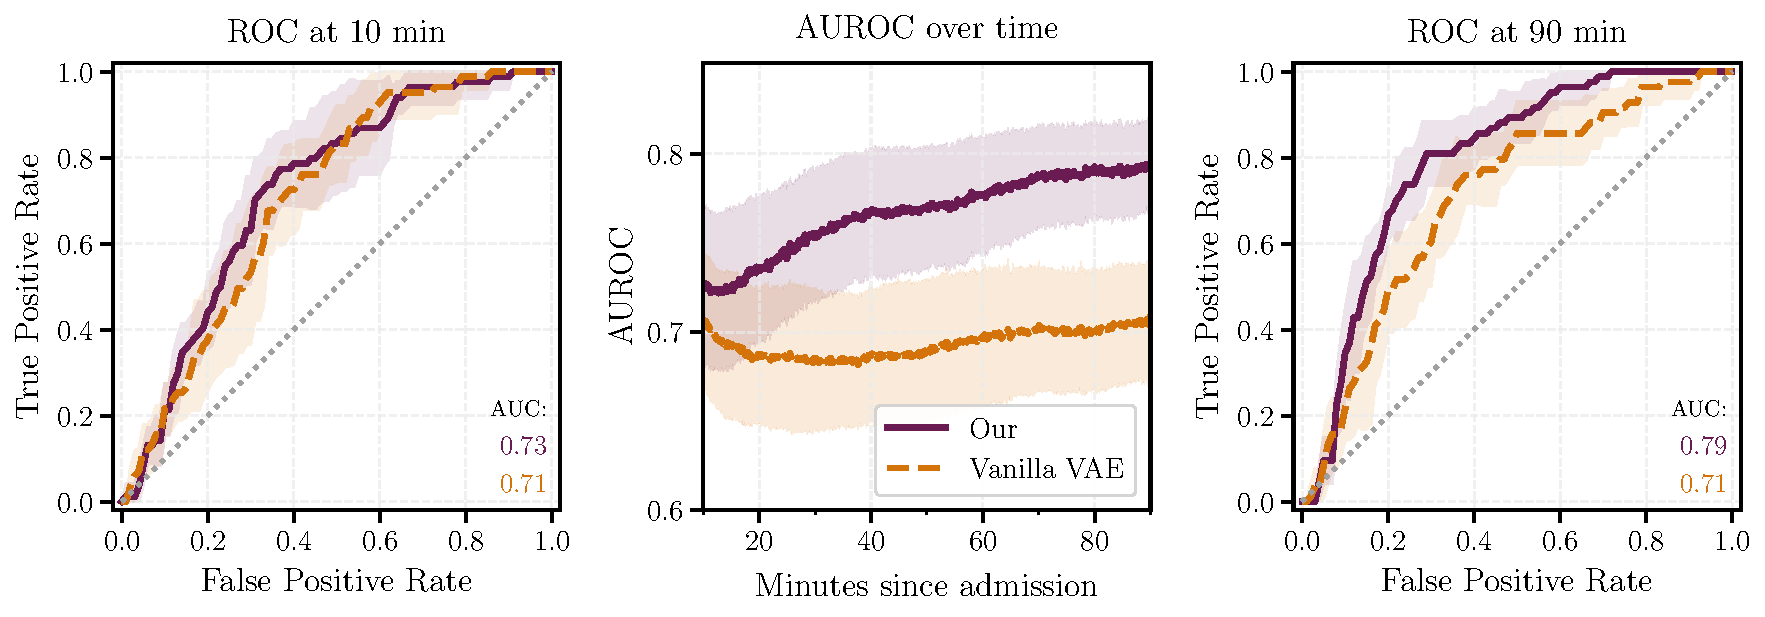
\includegraphics[width=0.95\textwidth]{figs/auroc_and_roc_comparison.pdf}
  \caption{Discrimination performance comparing the structured VAE with a vanilla VAE for encoding thermo-visual imaging, with all three modalities active in both settings. Receiver operating characteristic curves are shown at 10 and 90\,min after post-anaesthesia care unit admission. The middle panel shows AUROC trajectories from 10 to 90\,min.}
  \label{fig:auroc-roc-comparison}
\end{figure*}

\begin{figure*}[htbp]
  \centering
  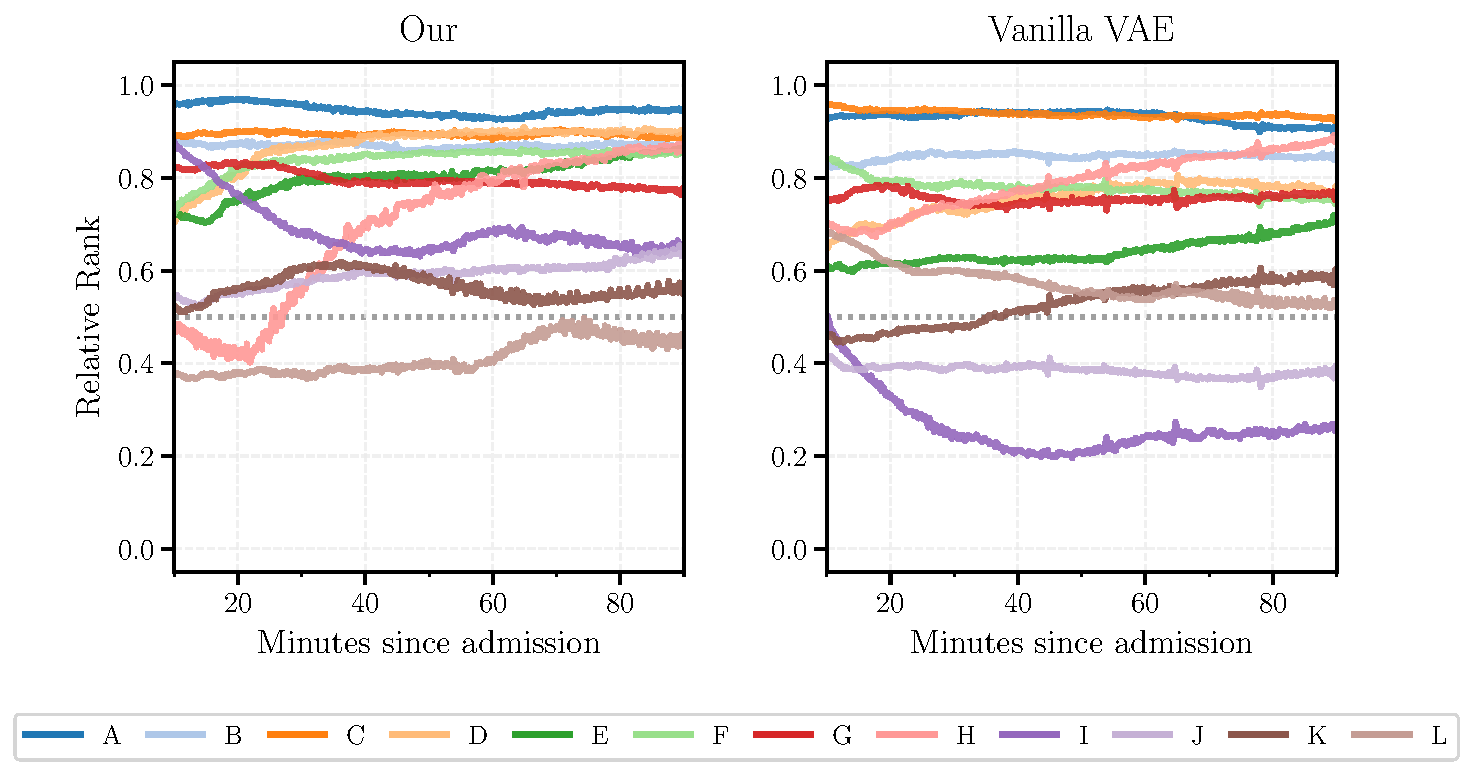
\includegraphics[width=\textwidth]{figs/patient_ranks_comparison.pdf}
  \caption{Temporal evolution of per-patient risk ranks for the structured VAE and a vanilla VAE, with electronic health records, physiological waveform data and thermo-visual imaging active in both settings. Each line traces the relative risk rank assigned to an individual neurological complication case across time.}
  \label{fig:patient-ranks-comparison}
\end{figure*}

\begin{figure*}[htbp]
  \centering
  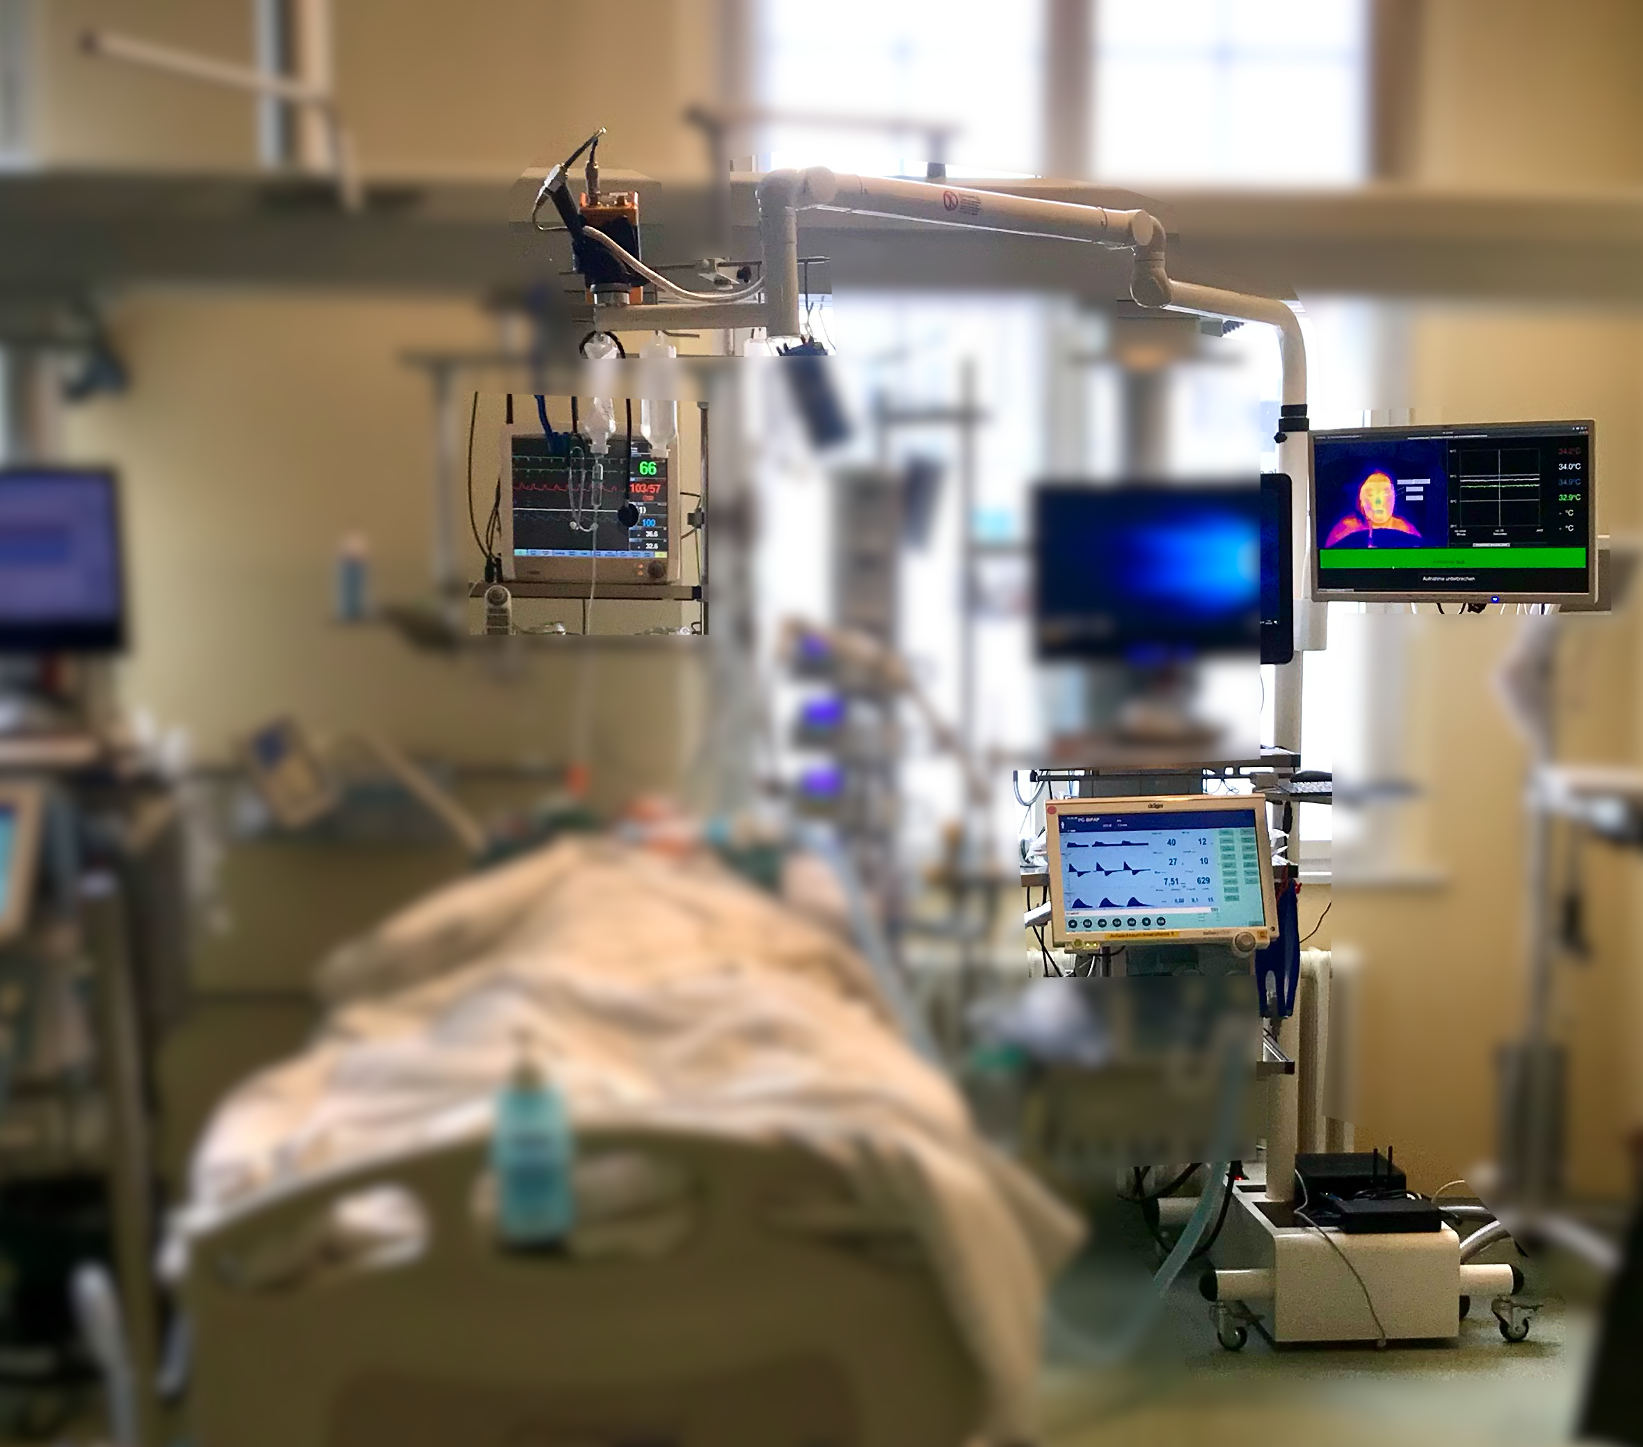
\includegraphics[width=0.95\textwidth]{figs/Setup.png}
  \caption{Bedside acquisition setup used to capture synchronised thermal and visual video, physiological waveform data and electronic health record data during the immediate postoperative post-anaesthesia care unit stay.}
  \label{fig:setup}
\end{figure*}

\end{document}